\documentclass[9pt, oneside, b5paper, openright]{memoir}
%\documentclass[9pt, twoside, openright, showtrims]{memoir}
\usepackage[b5paper, total={5in, 7in}]{geometry}
%\setstocksize{11in}{8in}
%\settrimmedsize{9in}{8in}{*}
%\settrims{0.7in}{0in}
%\settypeblocksize{7.5in}{6.3in}{*}
%\setlrmargins{.85in}{*}{*}
%\setulmargins{*}{.6in}{*}
%\setheadfoot{\onelineskip}{2\onelineskip}
%\setheaderspaces{*}{2\onelineskip}{*}
%\checkandfixthelayout

\makeatletter
\DeclareOldFontCommand{\rm}{\normalfont\rmfamily}{\mathrm}
\DeclareOldFontCommand{\sf}{\normalfont\sffamily}{\mathsf}
\DeclareOldFontCommand{\tt}{\normalfont\ttfamily}{\mathtt}
\DeclareOldFontCommand{\tt}{\smallfont\ttfamily}{\texxttt}
\DeclareOldFontCommand{\bf}{\normalfont\bfseries}{\mathbf}
\DeclareOldFontCommand{\it}{\normalfont\itshape}{\mathit}
\DeclareOldFontCommand{\sl}{\normalfont\slshape}{\@nomath\sl}
\DeclareOldFontCommand{\sc}{\normalfont\scshape}{\@nomath\sc}
\makeatother

% \usepackage{xcolor, calc, graphicx, soul, fourier, verbments, makeidx, mflogo}
\usepackage{xcolor, calc, graphicx, soul, float, makeidx, mflogo,
  pstricks, minitoc, amsmath, amssymb, pst-poly, longtable, tikz, titlesec,
  scalerel, stackengine, microtype, enumitem, wrapfig, mathtools}
% make minimum size of math font bigger
\let\frac\dfrac
\usetikzlibrary{shapes, arrows, calc}
\graphicspath{ {./images/} }
% Define block styles
\tikzstyle{decision} = [diamond, draw,
  text width=4.5em, text badly centered, node distance=3cm, inner sep=0pt]
\tikzstyle{startstop} = [rectangle, draw,
  text width=5em, text centered, rounded corners, minimum height=2em]
\tikzstyle{line} = [draw, -latex']
\tikzstyle{cloud} = [draw, ellipse, node distance=3cm,
  minimum height=0.5cm]
\tikzstyle{io} = [trapezium, trapezium left angle=70, trapezium right
  angle=110, minimum width=0.5cm, minimum height=0.5cm, text centered, draw=black,
]
\tikzstyle{process} = [rectangle, minimum width=1cm, minimum height=0.5cm, text
  centered, draw=black]
\tikzstyle{arrow} = [->,>=stealth]

\newcommand\dangersign[1][2ex]{%
  \renewcommand\stacktype{L}%
  \scaleto{\stackon[1.3pt]{\color{red}$\triangle$}{\tiny !}}{#1}%
}

\let\footruleskip\undefined
\usepackage{fancyhdr}
\usepackage{fancyvrb}
\pagestyle{fancy}
\usepackage[shellescape, latex]{gmp}
\showtrimson

\definecolor{niceblack}{rgb}{.1, .1, .1}
\definecolor{webred}{rgb}{.7,0,0}
\definecolor{webbg}{rgb}{1,.8,.2}
\definecolor{bootstrapurl}{rgb}{0,.5,.75}
\definecolor{nicered}{rgb}{.7,0,0}
\definecolor{nicegreen}{rgb}{.129,.447,.149}
\definecolor{niceblue}{rgb}{0, 0, .6}
\definecolor{niceyellow}{rgb}{1,1,.95}
\color{niceblack}
\usepackage[colorlinks]{hyperref}
\hypersetup{%
  pdftitle={Algebra},
  pdfauthor={Shiv S. Dayal},
  bookmarksnumbered,
  pdfstartview={FitH},
  urlcolor=cyan,
  linkcolor=cyan,
}%
\setlength{\tabcolsep}{10pt}
\renewcommand{\arraystretch}{1.5}

\renewcommand{\chaptermark}[1]{%
  \markboth{#1}{}}
\renewcommand{\sectionmark}[1]{%
  \markright{#1}{}}

\makeatletter
\newlength\dlf@normtxtw
\setlength\dlf@normtxtw{\textwidth}
\def\myhelvetfont{\def\sfdefault{mdput}}
\newsavebox{\feline@chapter}
\newcommand\feline@chapter@marker[1][4cm]{%
  \sbox\feline@chapter{%
    \resizebox{!}{#1}{\fboxsep=1pt%
      \colorbox{cyan}{\color{white}\bfseries\sffamily\thechapter}%
  }}%
  \rotatebox{90}{%
    \resizebox{%
      \heightof{\usebox{\feline@chapter}}+\depthof{\usebox{\feline@chapter}}}%
              {!}{\scshape\so\@chapapp}}\quad%
  \raisebox{\depthof{\usebox{\feline@chapter}}}{\usebox{\feline@chapter}}%
}
\newcommand\feline@chm[1][4cm]{%
  \sbox\feline@chapter{\feline@chapter@marker[#1]}%
  \makebox[0pt][l]{% aka \rlap
    \makebox[1cm][r]{\usebox\feline@chapter}%
}}
\makechapterstyle{daleif1}{
  \renewcommand\chapnamefont{\normalfont\HUGE\sffamily\scshape\raggedleft\so}
  \renewcommand\chaptitlefont{\normalfont\HUGE\sffamily\bfseries\scshape\color{cyan}}
  \renewcommand\chapternamenum{}
  \renewcommand\printchaptername{}
  \renewcommand\printchapternum{\null\hspace*{4.5in}\feline@chm[1cm]\par}
  \renewcommand\afterchapternum{\par\vskip\midchapskip}
  \renewcommand\printchaptertitle[1]{\chaptitlefont\raggedleft ##1\par}
}
\makeatother
\chapterstyle{daleif1}

\title{\sffamily\color{cyan}\HUGE{\textbf{A Variable in Algebra}}}
\author{\vspace*{1cm}\LARGE{Shiv S. Dayal}}
\date{}
\titleformat{\section}
  {\normalfont\sffamily\Large\bfseries\color{cyan}}
  {\thesection}{0.2em}{}
\titleformat{\subsection}
  {\normalfont\sffamily\large\bfseries\color{cyan}}
  {\thesection}{0.2em}{}
\titleformat{\subsubsection}
  {\normalfont\sffamily\large\bfseries\color{cyan}}
  {\thesection}{0.2em}{}
\titleformat{\subsubsubsection}
  {\normalfont\sffamily\bfseries\color{cyan}}
  {\thesection}{0.2em}{}
\renewcommand{\ttdefault}{pcr}
\setlength{\parskip}{1em}
\renewcommand{\rmdefault}{ptm}
\renewcommand{\rmdefault}{phv}
\usepackage{fontspec}
%\setmainfont{Roboto}
%\setmonofont[Ligatures=TeX,Scale=.90]{Courier}
\setsansfont{Roboto}
\renewcommand{\contentsname}{Table of Contents}
\makeindex
\setcounter{secnumdepth}{5}
\usepackage{etoolbox}
\makeatletter
\preto{\@verbatim}{\topsep=0pt \partopsep=0pt }
\makeatother
\begin{document}
\minitoc
\minilof
\minilot
\maketitle
\thispagestyle{empty}
\pagestyle{empty}
\vfill
\newpage
\vspace*{5in}
Build Date: \today
\vspace*{0.2in}

Copyright, \copyright~ Shiv Shankar Dayal, 2011-2023. All rights reserved.\\\\
Permission is granted to copy, distribute and/or modify this document under the
terms of the GNU Free Documentation License, Version 1.3 or any later version
published by the Free Software Foundation; with no Invariant Sections, no
Front-Cover Texts, and no Back-Cover Texts. A copy of the license is included
in the section entitled ``GNU Free Documentation License''.
\newpage
\vspace*{2in}
\begin{center}
  \Large \it Dedicated to my family\\and Free Software Community
\end{center}
\vspace*{1cm}
\begin{center}
  \large When you take an action think of the poorest person you have seen and evaluate how
  your action will benefit that person.
\end{center}
\newpage
\setcounter{page}{1}
\pagenumbering{roman}
\tableofcontents
% \newpage
% \listofpyglistings
\newpage
\pagestyle{fancy}
\frontmatter
\setcounter{page}{1}
\pagenumbering{roman}
\chapter{Preface}
This is a book on algebra, which, covers basics of algebra till high school level. It covers the most essential topics to take up a
bachelor's course where knowledge of algebra is required. There is no specific purpose for writing this book. This is a book for
self study and is not recommended for courses in schools and universities. I will try to cover as much as I can and will keep
adding new material over a long period. I have no interest in writing a book in a fixedly way which serves a university or college
course as I have always loved freedom. Life, freedom and honor in that order are important.

Algebra is probably one of the most fundamental subjects in Mathematics as further study of subjects like trigonometry, coordinate
geometry and rest all depend on it. That is the primary reason I have chosen it to be the first subject in mathematics to be dealt
with. It is very important to understand algebra for the readers if they want to advance further in mathematics.

\section*{Why I Wrote This Book?}
I wrote this book for myself! I did not write it for anybody else. My knowledge, which I have acquired by reading books written by
many great mathematicians and authors and interactions with many intelligent people, is what has been put in the book. I have just
tried to add my flavor to it. Think of it as notes for me. Just that I like to organize my notes so it has taken form of a book and
nothing more. If you benefit from this then that is a pure coincidence and not intentional at all.

\section*{How to Read This Book?}
No I will not simply tell that you must solve the problems. My advice would be more detailed. Every chapter will have theory. Read
that first. Make sure you understand that. Of course, you have to meet the prerequisites for the book. Then, go on and try to solve
the problems. In this book, there are no pure problems. Almost all have answers except those which are of similar kind and
repetitive in nature for the sake of practice. If you can solve the problem then all good else look at the answer and try to
understand that. Then, few days later take on the problem again. If you fail to understand the answer you can always email me with
your work and I will try to answer to the best of my ability. However, if you have a local expert seek his/her advice first. Just
that email is bad for mathematics.

Note that mathematics is not only about solving problems. If you understand the theory well, then you will be able to solve
problems easily. However, problems do help enforce with the enforcement of theory in your mind.

I am a big fan of old MIR publisher's problem books, so I emphasize less on theory and more on problems. I hope that you find
this style much more fun as a lot of theory is boring. Mathematics is about problem solving as that is the only way to
enforce theory and find innovtive techniques for problem solving.

\section*{Who Should Read This Book?}
Since this book is written for self study anyone with interest in algebra can read it. That does not mean that school or college
students cannot read it. You need to be selective as to what you need for your particular requirements. This is mostly high school
course with a little bit of lower classes' course thrown in with a bit of detail here and there.

\section*{Prerequisite}
You should have knowledge till grade 10th course. Attempt has been made to keep it simple and give as much as background to the
topic which is reasonable and required. However, not everything will be covered below grade 10.

\section*{Goals for Readers}
The goal of for reading this book is becoming proficient in solving simple and basic problems of algebra. Another goal would be to
be able to study other subjects which require this knowledge like trigonometry or calculus or physics or chemistry or other
subjects. If you can solve 95\% problems after 2 years of reading this book then you have achieved this goal.

All of us possess a certain level of intelligence. At average any person can read this book. But what is most important is you have
to have interest in the subject. Your interest gets multiplied with your intelligence and thus you will be more capable than you
think you can be. One more point is focus and effort. It is not something new which I am telling but I am saying it again just to
emphasize the point. Trust me if you are reading this book for just scoring a nice grade in your course then I have failed in my
purpose of explaining my ideas.

Also, if you find this book useful feel free to share it with others without hesitation as it is free as in freedom. There are no
conditions to share it.

\section*{Acknowledgements}
I am in great debt of my family and free software community because both of
these groups have been integral part of my life. Family has prvided direct
support while free software community has provided the freedom and freed me
from the slavery which comes as a package with commercial software. I am
especially grateful to my wife, son and parents because it is their time which
I have borrowed to put in the book. To pay my thanks from free software
community  I will take one name and that is Richard Stallman who started all
this  and is still fighting this never-ending war. When I was doing the Algebra
book then I realized how difficult it is to put Math on web in HTML format and
why Donald Knuth wrote \TeX{}. Also, \TeX{} was one of the first softwares to
be released as a free software.

Now as this book is being written using \LaTeX{} so obviously Leslie Lamport
and all the people involved with it have my thanks along with Donald Knuth. I
use Emacs with Auctex and hope that someday I will use it in a much more
productive way someday.

I have used Asymptote and tikz for drawing all the diagrams. Both are wonderful
packages and works very nicely. Asymptote in particular is very nice for 3d-drawings and linear equation solving.

I would like to thank my parents, wife and son for taking out their fair share
of time and the support which they have extended to me during my bad
times. After that I would like to pay my most sincere gratitude to my teachers
particularly H. N. Singh, Yogendra Yadav, Satyanand Satyarthi, Kumar Shailesh
and Prof. T. K. Basu. Now is the turn of people from software community. I must
thank the entire free software community for all the resources they have
developed to make computing better. However, few names I know and here they
go. Richard Stallman is the first, Donald Knuth, Edger Dijkstra, John von Neumann after that as their lives have strong influence in
how I think and base my life on.

I am not a native English speaker and this book has just gone through one pair
of eyes therefore chances are high that it will have lots of errors(particularly with commas and spelling mistakes). At the
same time it may contain lots of technical errors. Please feel free to drop me
an email at
\href{mailto:shivshankar.dayal@gmail.com}{shivshankar.dayal@gmail.com} where I
will try to respond to each mail as
much as possible. Please use your real names in email not something like
coolguy. If you have more problems which you want to add it to the book please send
those by email or create a PR on github. The github url is \url{https://github.com/shivshankardayal/Algebra-Latex}.
\begin{flushright}
Shiv Shankar Dayal\\
Nalanda,\\
India, 2015
\end{flushright}

\newpage
\mainmatter
\pagenumbering{arabic}
\part{Theory and Problems}
\chapter{Logarithm}
\textbf{Definition:} A number $x$ is called the logarithm of a number $y$ to the base $b$ if $b^x = y$, where $b > 0, b\neq 1, y > 0$.

\noindent Mathematically, it is represented by the equation $\log_b y = x$ or $b^x = y$.

\textbf{Notes:}
\begin{enumerate}
\item The conditions $b>0, b\neq 1$ and $y>0$ are necessary in the definition of logarithm.
\item When $b=1$ suppose logarithm is defined, and we have to find the value of $\log_1y$. Let
  $\log_1y=x\Rightarrow 1^x=y\Rightarrow 1=y$.

  If $\log_12$ is defined then $1 = 2$. So we see that $b = 1$ leads to meaningless results. Similarly, it is true for $b \neq 1$.
\item Similarly if $y < 0$, then $b^x = y$, which is meaningless as L.H.S. is positive while R.H.S. is negative.
\item Let the condition to be true when $b = 0$. Thus, $0^x = y\Rightarrow 0 = y$. Thus, if $\log_0 2$ is defined then $0 =
  2$. Hence, our assumption leads to failure.
\item No number can have two different logarithms to a given base. Assume that a number $N$ has two different logarithms $x$ and
  $y$ with base $b$. Then, $\log_b N = x$ and $\log_b N = y$

  $\Rightarrow N = b^x$ and $N = b^y$

  $\Rightarrow b^x = b^y \Rightarrow x = y$
\item When the number or base is negative the value of logarithm comes out to be a complex number with non-zero imaginary part.

  Let $\log_e(-5) = x \Rightarrow \log_e(5.e^{i\pi}) = x$ (In complex numbers $e^{i\pi} = -1$)

  $x = \log_e5 + i\pi$
\end{enumerate}

\section{Important Results}
\begin{enumerate}
\item $\log_b 1 = 0$

  \textbf{Proof:} Let $\log_b 1 = x\Rightarrow b^x = 1 \Rightarrow x = 0$
\item $\log_b b = 1$

  \textbf{Proof:} Let $\log_b b = x \Rightarrow b^x = b \Rightarrow x = 1$
\item $b^{\log_b N} = N$

  \textbf{Proof:} Let $\log_b N = x\Rightarrow b^x = N \Rightarrow b^{\log_b N} = N$
\end{enumerate}
\section{Important Formulas}
\begin{enumerate}
\item $\log_b(x.y) = \log_bx + \log_by, (x>0, y>0)$

  \textbf{Proof:} Let $\log_bx = m \Rightarrow b^m = x$. Similarly, $b^n = y$

  $xy = b^{m + n} = b^o$ (say)

  $m + n = o \Rightarrow \log_b(x.y) = \log_bx + \log_by$

  \textbf{Corollary:} $\log_b(xyz) = \log_bx + \log_by + \log_bz$

  If $x, y < 0,$ then $\log_b(x.y) = \log_b|x| + \log_b|y|$
\item $\log_b\left(\frac{x}{y}\right) = \log_b x - \log_b y, (x, y > 0)$

  \textbf{Proof:} Let $\log_bx = m \Rightarrow b^m = x$ and $\log_by = n \Rightarrow b^n = y$

  $\frac{x}{y} = b^{m - n}$ and $\log_b\left(\frac{x}{y}\right) = o \Rightarrow b^o = \frac{x}{y}$

  $\Rightarrow m - n = o \Rightarrow \log_b\left(\frac{x}{y}\right) = \log_b x - \log_b y$

  $\log_b\left(\frac{x}{y}\right) = \log_b|x| - \log_b|y|, (x, y < 0)$
\item $\log_bN^k = k\log_b N$

  \textbf{Proof:} Let $\log_bN = x \Rightarrow b^x = N$

  Let $\log_bN^k = y \Rightarrow b^y = N^k \Rightarrow b^y = b^{kx} \Rightarrow y = kx$

  $\Rightarrow \log_bN^k = k\log_b N$
\item $\log_ba = \log_ca\log_bc$

  \textbf{Proof:} Let $\log_ba = x \Rightarrow b^x = a$

  $\log_ca = y \Rightarrow c^y = a$

  $\log_bc = z \Rightarrow b^z = c$

  $b^x = a = c^y = b^{yz} \Rightarrow x = yz \Rightarrow \log_ba = \log_ca\log_bc$

  Alternatively, we can also write it as $\log_ba = \frac{\log_ca}{\log_cb}$
\item $\log_{b^k}N = \frac{1}{k}\log_bN[b > 0]$

  \textbf{Proof:} From previous item we can infer that $\log_{b^k}N = \frac{\log N}{\log b^k} = \frac{1}{k}\log_bN$

  $\log_{b^k}N = \frac{1}{k}\log_{|b|}N[b< 0, k = 2m, m\in N]$
\item $\log_ba = \frac{1}{\log_ab}$

  \textbf{Proof:} Let $\log_ba = x \Rightarrow b^x = a$

  Also let $\log_ab = y \Rightarrow a^y = b = a^{xy} \Rightarrow xy = 1$

  $\Rightarrow \log_ba = \frac{1}{\log_ab}$
\end{enumerate}

\section{Bases of Logarthims}
There are two popular bases for logarithms. Common base is $10$ and another is $e$. When base is $10$, logarithm is known as
\textit{common logarithm} and when base is $e$, logarithm is known as \textit{natural} or \textit{Napierian logarithm}.

$\log_{10}x$ is also written as $lg~x$ and $\log_ex$ as $ln~x$.

\section{Characteristics and Mantissa}
Typically a logarithm will have an integral part and a fractional part. The integral part is called \textit{characteristics} and
fractional part is called \textit{mantissa}.

For example, if $\log x = 4.7$ then $4$ is characteristics and $.7$ is mantissa of logarithm. If characteristics is less that zero
then at times it is written with a bar above it. For example, $\log x=-5.3=\overline{5}.3$

As you can easily figure out the number of possitive integers having base $b$ and characteristics $n$ is $b^{n + 1} - b^n$.

\section{Inequality of Logarithms}
If $b > 1$ and $\log_bx_1 > \log_bx_2$ then $x_1 > x_2$. If $b < 1$ and $\log_bx_1 > \log_bx_2$ then $x_1 < x_2$.

\section{Expansion of Logarithm and Its Graph}
The logarithm series is given below:

$$\log(1 + x) = x - \frac{x^2}{2} + \frac{x^3}{3} - \frac{x^4}{4} + \ldots$$

\begin{figure}[H]
\begin{center}
  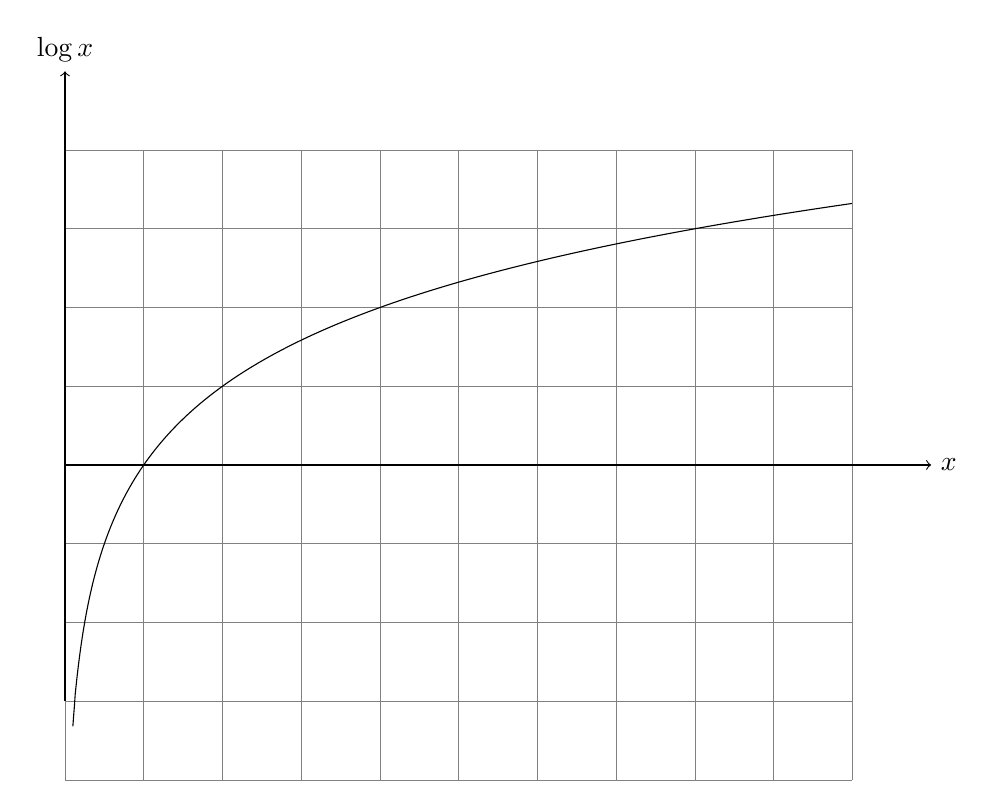
\begin{tikzpicture}
    \draw [help lines] (0,-4) grid [step=1] (10,4);
    \draw (0,0) -- (10,0);
    \draw[->] (0, 0) -- (11, 0) node[right] {$x$};
    \draw[->] (0, -3) -- (0, 5) node[above] {$\log x$};
    \draw plot [domain=0.1:10,samples=1000] (\x,{log2(\x)});
  \end{tikzpicture}
  \caption{Graph of $\log 2$}
\end{center}
\end{figure}

So we can see that rate of increment of logarithm function decreases. Rate of increment of logarithm function is given by
$\frac{1}{x}$ at any point $x$, as we will learn when we study Calculus and derivatives.

\section{Problems}
\begin{enumerate}
\item Find the value of $x$, where $\log_{\sqrt{8}} x = \frac{10}{3}$.
\item Prove that $\log_ba.\log_cb.\log_ac = 1$.
\item Prove that $\log_3\log_2\log_{\sqrt{5}}625 = 1$.
\item If $a^2 + b^2 = 23ab$, then prove that $\log\tfrac{a + b}{5} = \frac{1}{2}(\log a + \log b)$.
\item Prove that $7\log\frac{16}{15} + 5\log\frac{25}{24} + 3\log\frac{81}{80} = \log 2$.
\item Find the value of $\log\tan1^\circ + \log\tan2^\circ + \ldots + \log\tan89^\circ$.
\item Evaluate $\log_9\tan\frac{\pi}{6}$.
\item Evaluate $\frac{\log_{a^2}b}{\log_{\sqrt{a}}b^2}$.
\item Evaluate $\log_{\sqrt{5}}.008$.
\item Evaluate $\log_{2\sqrt{3}}144$.
\item Prove that $\log_3\log_2\log_{\sqrt{3}}81 = 1$.
\item Prove that $\log_ax\log_by = \log_bx\log_ay$.
\item Prove that $\log_2\log_2\log_216 = 1$.
\item Prove that $\log_ax = \log_bx\log_cb\ldots\log_nm\log_an$.
\item Prove that $a^x = 10^x\log_{10}a$.
\item If $a^2 + b^2 = 7ab$, prove that $\log\left\{\tfrac{1}{3}(a + b)\right\} = \frac{1}{2}(\log a + \log b)$.
\item Prove that $\frac{\log a\log_ab}{\log b\log_ab} = -\log_ab$.
\item Prove that $\log(1 + 2 + 3) = \log 1 + \log 2 + \log 3$.
\item Prove that $2\log(1 + 2 + 4 + 7 + 14) = \log 1 + \log 2 + \log 4 + \log 7 + \log 14$.
\item Prove that $\log 2 + 16\log\frac{16}{15} + 12\log\frac{25}{24} + 7\log\frac{81}{80} = 1$.
\item Simplify $\frac{\log_911}{\log_513}\div\frac{\log_311}{\log_{\sqrt{5}}}13$.
\item Simplify $3^{\sqrt{\log_32}} - 2^{\sqrt{\log_23}}$.
\item Find the least integer $n$ such that $7^n > 10^5$, given that $\log_{10}343 = 2.5353$.
\item If $a, b, c$ are in G.P., prove that $\log_ax, \log_bx, \log_cx$ are in H.P.
\item Prove that $\log\sin8x = 3\log2 + \log\sin x + \log\cos x + \log\cos2x + \log\cos4x$.
\item If $x = \log_{2a}a, y = \log_{3a}2a$ and $z = \log_{4a}3a$ then prove that $xyz + 1 = 2yz$.
\item If $a$ and $b$ are the lengths of the sides and $c$ be the length of the hypotenuse of a right-angle triangle and $c - b \neq
  1$ and $c + b\neq 1$, prove that $\log_{c + b}a + \log_{c - b}a = 2\log_{c + b}a\log_{c - b}a$.
\item If $\frac{\log x}{y - z} = \frac{\log y}{z - x} = \frac{\log z}{x - y}$, then prove that $x^xy^yz^z = 1$.
\item If $\frac{yz\log(yz)}{y + z} = \frac{zx\log(zx)}{z + x} = \frac{xy\log(xy)}{x + y}$, prove that $x^2 = y^y = z^2$.
\item Prove that $(yz)^{\log y - \log z}(zx)^{\log z - \log x}(xy)^{\log x - \log y} = 1$.
\item Prove that $\frac{1}{\log_2N} + \frac{1}{\log_3N} + \ldots + \frac{1}{\log_{1988}N} = \frac{1}{\log_{1988!}N}$.
\item If $0<x<1$, prove that $\log(1 + x) + \log(1 + x^2) + \log(1 + x^4) + \ldots$ to $\infty = -\log(1 - x)$.
\item Find the sum of the series $\frac{1}{\log_2a} + \frac{1}{\log_4a} + \ldots$ up to $n$ terms.
\item If $\log_410 = x, \log_220 = y$ and $\log_58 = z$, prove that $\frac{1}{x + 1} + \frac{1}{y + 1} + \frac{1}{z + 1} = 1$.
\item If $x = \log_abc, y = \log_bca, z = \log_cab$, prove that $\frac{1}{x + 1} + \frac{1}{y + 1} + \frac{1}{z + 1} = 1$.
\item Prove that $\frac{1}{1 + \log_ba + \log_bc} + \frac{1}{1 + \log_ca + \log_cb} + \frac{1}{1 + \log_ab + \log_ac} = 1$.
\item Prove that $x^{\log y - \log z}y^{\log z - \log x}z^{\log x - \log y} = 1$.
\item If $\frac{\log a}{y - z} = \frac{\log b}{z - x} = \frac{\log c}{x - y}$, prove that $a^xb^yc^z = 1$.
\item If $\frac{x(y + z - x)}{\log x} = \frac{y(z + x - y)}{\log y} = \frac{z(x + y - z)}{x - y}$, prove that $y^zz^y = z^xx^z =
  x^yy^x$.
\item If $\frac{\log a}{b - c} = \frac{\log b}{c - a} = \frac{\log c}{a - b},$ prove that $a^{b + c}b^{c + a}c^{a + b} = 1$.
\item If $\frac{\log x}{q - r} = \frac{\log y}{r - p} = \frac{\log z}{p - q}$, prove that $x^{q + r}y^{r + p}z^{p + q} =
  x^py^qz^r$.
\item If $y = a^{\frac{1}{1 - \log _ax}}$ and $z = a^{\frac{1}{1 - \log_ay}}$, prove that $x = a^{\frac{1}{1 - \log_az}}$.
\item Let $f(x) = \frac{1}{1 - \log_ex}$, $f(y) = e^{f(z)}$ and $z = e^{f(x)}$, prove that $x = e^{f(y)}$.
\item Show that $\frac{1}{\log_2n} + \frac{1}{\log_3n} + \frac{1}{\log_4n} + \ldots + \frac{1}{\log_{43}n} =
  \frac{1}{\log_{43!}n}$.
\item Show that $2(\log a + \log a^2 + \log a^3 + \ldots + \log a^n) = n(n + 1)\log a$.
\item Find the number of digits in $12^{12}$, without actual computation. [Given $\log 2 = 0.301$ and $\log 3 = 0.477$]
\item How many positive integers have a characteristics of $2$ when base is $3$.
\item Prove that $\log_ax\log_by = \log_bx\log_ay$.
\item If $a, b, c$ are in G.P., prove that $\log_ax, \log_bx, \log_cx$ are in H.P.
\item How many zeros are there between the decimal point and first significant digit in $0.0504^{10}?$ Given $\log 2 = 0.301, \log
  3 = 0.477, \log 7 = 0.845$.
\item Find the number of digits in $72^{15}$ without actual computation. Given $\log 2 = 0.301$ and $\log  3 = 0.477$.
\item How many positive integers have characteristics $2$ when base is $5$?
\item If $\log 2 = 0.301$ and $\log 3 =0.477$, find the number of digits in $3^{15}\times 2^{10}$.
\item If $\log 2 = 0.301$ and $\log 3 =0.477$, find the number of digits in $6^{20}$.
\item If $\log 2 = 0.301$ and $\log 3 =0.477$, find the number of digits in $5^{25}$.
\item Solve $\log_a[1 + \log_b\{1 + \log_c(1 + \log_px)\}] = 0$.
\item Solve $\log_7\log_5(\sqrt{x + 5} + \sqrt{x}) = 0$.
\end{enumerate}

\noindent Solve the following equations:

\begin{enumerate}[resume]
\item $\log_2x + \log_4(x + 2) = 2$.
\item $\log_{x + 2}x + \log_x(x + 2) = \frac{5}{2}$.
\item $\log(x + 1) = 2\log x$.
\item $2\log_xa + \log_{ax}a + 3\log_{a^2x}a = 0.$ Given $a > 0$.
\item $x + \log_{10}(1 + 2^x) = x\log_{10}5 + \log_{10}6$.
\item $x^{\tfrac{3}{4}(\log_2x)^2 + \log_x{2 - \tfrac{5}{4}}} = \sqrt{2}$.
\item $(x^2 + 6)^{\log_3x} = (5x)^{\log_3x}$.
\item $(3 + 2\sqrt{2})^{x^2 - 6x + 9} + (3 - 2\sqrt{2})^{x^2 - 6x + 9} = 6$.
\item $\log_8\left(\tfrac{8}{x^2}\right)\div(\log_8x)^2 = 3$.
\item $\sqrt{\log_2(x)^4} + 4\log_4\sqrt{\tfrac{2}{x}} = 2$.
\item $2\log_{10}x - \log_x0.01 = 5$.
\item $\log_{\sin x}2\log_{\cos x}2 + \log_{\sin x}2 + \log_{\cos x}2 = 0$.
\item $2^{x + 3} + 2^{x+2} + 2^{x + 1} = 7^x + 7^{x - 1}$.
\item $\log_{\sqrt{2}\sin x}(1 + \cos x) = 2$.
\item $\log_{10}[198 + \sqrt{x^3 - x^2 - 12x + 36}] = 2$.
\item If $\log 2 = 0.30103$ and $\log 3 = 0.47712,$ solve the equation $2^x3^{2x} - 100 = 0$.
\item $\log_x3\log_{\frac{x}{3}}3 + \log_{\frac{x}{81}}3 = 0$.
\item $\log_{(2x + 3)}(6x^2 + 23x + 21) = 4 - \log_{(3x + 7)}(4x^2 + 12x + 9)$.
\item $\log_2(x^2 - 1) = \log_{\frac{1}{2}}(x - 1)$.
\item $\log_5\left(5^{\tfrac{1}{x} + 125}\right) = \log_56 + 1 + \frac{1}{2x}$.
\item $\log_{100}|x + y| = \frac{1}{2}$ and $\log_{10}y - \log_{10}|x| = \log_{100}4$.
\item $2\log_2\log_2x + \log_{\tfrac{1}{2}}\log_2(2\sqrt{2}x) = 1$.
\item $\log_{\tfrac{3}{4}}\log_8(x^2 + 7) + \log_{\tfrac{1}{2}}\log_{\tfrac{1}{4}}(x^2 + 7)^{-1} = 2$.
\item $\log_{10}x + \log_{10}x^{\tfrac{1}{2}} + \log_{10}x^{\tfrac{1}{4}} + \ldots$ to $\infty = y$ and $\frac{1 + 3 + 5 + \ldots +
  (2y - 1)}{4 + 7 + 10 + \ldots + (3y + 1)} = \frac{20}{7\log_{10}x}$.
\item $18^{4x - 3} = (54\sqrt{2})^{3x - 4}$.
\item $4^{\log_93} + 9^{\log_24} = 10^{\log_x83}$.
\item $3^{4\log_9(x + 1)} = 2^{2\log_2(x + 3)}$.
\item $\frac{6}{5}a^{\log_ax\log_{10}a\log_a5} - 3^{\log_{10}\tfrac{x}{10}} = 9^{\log_{100}x + \log_42}$.
\item $2^{3x + \frac{1}{2}} + 2^{x + \frac{1}{2}} = 2^{\log_26}$.
\item $(5 + 2\sqrt{6})^{x^2 - 3} + (5 - 2\sqrt{6})^{x^2 - 3} = 10$.
\item For $x> 1$, show that $2\log_{10x}x - \log_x{.01}\geq 4$.
\item Show that $|\log_b a + \log_ab| > 2$.
\item Solve $\log_{0.3}(x^2 + 8) > log_{0.3}9x$.
\item Solve $\log_{x - 2}(2x - 3) > \log_{x - 2}(24 - 6x)$.
\item Find the interval in which $x$ will lie if $\log_{0.3}(x - 1) < \log_{0.09}(x - 1)$.
\item Solve $\log_{\tfrac{1}{2}}x \geq \log_{\tfrac{1}{3}}x$.
\item Solve $\log_{\tfrac{1}{3}}\log_4(x^2 - 5) > 0$.
\item Solve $\log(x^2 -2x -2)\leq 0$.
\item Solve $\log_2^2(x-1)^2 - \log_{0.5}(x - 1) > 5$.
\item Prove that $\log_217\log_{\tfrac{1}{5}}2\log_3\tfrac{1}{5} > 2$.
\item Show that $\log_{20}3$ lies between $\frac{1}{2}$ and $\frac{1}{3}$.
\item Show that $\log_{10}2$ lies between $\frac{1}{4}$ and $\frac{1}{3}$.
\item Solve $\log_{0.1}(4x^2 - 1) > \log_{0.1}3x$.
\item Solve $\log_2(x^2 - 24) > \log_25x$.
\item Show that $\frac{1}{\log_3\pi} + \frac{1}{\log_4\pi} > 2$.
\item Without actual computation find greater among $(0.01)^{\tfrac{1}{3}}$ and $(0.001)^{\tfrac{1}{5}}$.
\item Without actual computation find greater among $\log_23$ and $\log_311$.
\item Solve $\log_3(x^2 + 10) > \log_37x$.
\item Solve $x^{\log_{10}x} > 10$.
\item Solve $\log_2x\log_{2x}2log_24x > 1$.
\item Solve $\log_2x\log_32x + \log_3x\log_24x > 0$.
\item Find the value of $\log_{12}60$ if $\log_630 = a$ and $\log_{15}24 = b$.
\item If $\log_ax, \log_bx$ and $\log_cx$ are in A.P. and $x\neq 1$, prove that $c^2 = (ac)^{\log_ab}$.
\item If $a = \log_{\tfrac{1}{2}}\sqrt{0.125}$ and $b = \log_3\left(\frac{1}{\sqrt{24} - \sqrt{17}}\right)$ then find whether $a >0,
  b> 0$.
\item Which one is greater among $\cos(\log_e\theta)$ and $\log_e(\cos\theta)$ if $e^{-\tfrac{\pi}{2}} < \theta < \frac{\pi}{2}$.
\item If $\log_2x + \log_2y \geq 6$, prove that $x + y\geq 16$.
\item If $a,b,c$ eb three distinct positive numbers, each different from $1$ such that $\log_ba\log_ca - \log_qaa + \log_ab\log_cb
  - \log_bb + \log_ac\log_bc - \log_cc = 0$.
\item If $y = 10^{\tfrac{1}{1 - \log x}}$ and $z = 10^{\tfrac{1}{1 - \log y}}$, prove that $x = 10^{\tfrac{1}{1 - \log z}}$.
\item If $n$ is a natural number such that $n = p_1^{a_1}p_2^{a_2}p_3^{a_3}\ldots p_k^{a_k}$ and $p_1, p_2, p_3, \ldots, p_k$ are
  distinct primes, then show that $\log n\geq k\log 2$.
\item The numbers $3, 3\log_yx, 3\log_zy, 7\log_xz$ form and A.P. then prove that $x^{18} = y^{21} = z^{28}$.
\item Prove that $\log_418$ is an irrational number.
\item If $x, y, z> 1$ are in G.P. then prove that $\frac{1}{1+ \ln x}, \frac{1}{1 + \ln y}, \frac{1}{1 + \ln z}$ are in H.P.
\item Find the value of $\log_{30}8$, if $\log_{30}3 = a$ and $\log_{30}5 = b$.
\item Find the value of $\log_{54}168$, if $\log_712 = a$ and $\log_{12}24 = b$.
\item If $a\neq 0$ and $\log_x(a^2 + 1) < 0$ then find the interval in which $x$ lies.
\item If $\log_{12}18 - a$ and $\log_{24}54=b$, prove that $ab + 5(a - b) = 1$.
\item If $a,b,c$ are in G.P., show that $\log_ax, \log_bx, \log_cx$ are in H.P.
\item If $a, a_1, a_2, \ldots, a_n$ are in G.P. and $b, b_1, b_2, \ldots, b_n$ in A.P. with positive terms and also the common
  difference of A.P. and common rations of G.P. are positive, show that there exists a system of logarithm for which $\log a_n -
  b_n = \log a - b$ for any $n$. Find the base of this system.
\item If $\log_32, \log_3(2^x - 5)$ and $\log_3\left(2^x - \frac{7}{2}\right)$ are in A.P., find the value of $x$.
\item Prove that $\log_27$ is an irraational number.
\item If $\log_{0.5}(x - 2) < \log_{0.25}(x - 2)$, then find the interval in which $x$ lies.
\end{enumerate}

\chapter{Complex Numbers}
By definition a complex number has two parts: a real part and an imaginary part. You already know about real numbers and know about
them. However, imaginary numbers is something different.
\section{Imaginary Numbers}
Imaginary numbers are called so because there cannot be physical representation of these quantities. Like we use real numbers for
counting physical objects we cannot do that with imaginary numbers. In real world, they do not exist. Square root of negative
numbers are called imaginary numbers. For example, $\sqrt{-1}, \sqrt{-2}. \sqrt{-3}, \ldots$ and so on.

We denote $\sqrt{-1}$ with the Greek symbol $\iota$, which stands for \textit{iota}. We also use English letters \textit{i} or
\textit{j} to represent this imaginary number. Clearly, $i^2 = -1, i^3 = -i, i^4 = 1$. If you examine carefully, you will find that
following holds true:

$$i^{4m} = 1, i^{4m + 1} = i, i^{4m + 2} = -1 \text{~and~} i^{4m +3} = -1, \forall m\in P$$

\dangersign \textbf{Gotcha:}

Consider the following:

$$1 = \sqrt{1} = \sqrt{-1*-1} = \sqrt{-1}*\sqrt{-1} = i*i = -1$$

However, the above result is wrong. The reason being is that for any two real numbers $a$ and $b, \sqrt{a}*\sqrt{b} = \sqrt{ab}$
holds good if and only if two numbers are either zero or positive. Also, $\sqrt{1}\neq \sqrt{-1*-1}$ because power of $-$ is
$\frac{1}{2}$ which results in $-1$.

\section{Definitions Related to Complex Numbers}
A complex number is written as $a + ib$ or $x + iy$ or $a + jb$ or $x + jb$. Here, $a, b, x, y$ are all real numbers. The complex
numbers itself is denoted by $z$. Therefore, we have $z = x + iy$. Here, $x$ is called the real part and is also denoted by $Re(z)$
and $y$ is called the imaginary part and is also denoted by $Im(z)$.

A complex number is purely real if its imaginary part or $y$ or $Im(z)$ is zero. Similarly, a complex number is purely imaginary if
its real part or $x$ or $Re(z)$ is zero. Clearly, as you can imagine that there can exist only one number which has both the parts
as zero and certainly that is $0$. That is, $0=0+i0$.

The set of all complex number is typically denoted by $C$. Two complex numbers $z_1$ and $z_2$ are said to be true if there real
parts are equal and imaginary parts are equal. That is if $z_1=x_1+iy_1$ and $z_2=x_2+iy_2$ then $x_1$ must be equal to $x_2$ and
similarly for imaginary part for two complex numbers to be equal.

\section{Simple Arithmetic Operations}
\subsection{Addition}
$(a + ib) + (c + id) = (a + c) + i(b + d)$
\subsection{Subtraction}
$(a + ib) - (c + id) = (a - c) + i(b - d)$
\subsection{Multiplication}
$(a + ib) * (c + id) = ac + ibc + iad + bdi^2 = (ac - bd) +i(bc + ad)$
\subsection{Division}
The complex number in denominator must not have both parts as zero. At least one part must be non-zero.

$$\frac{a + ib}{c + id} = \frac{(a + ib)(c - id)}{(c + id)(c -id)} = \frac{(ac + bd) + i(bc -ad)}{c^2+d^2}$$

\section{Conjugate of a Complex Number}
Let $z = x + iy$ be a complex number then its complex conjugate is a number with imaginary part made negative. It is written as
$\overline{z} = x - iy. \overline{z}$ is the typical representation for conjugate of a complex number $z$.

\subsection{Properties of Conjugates}
\begin{enumerate}
\item $z_1 = z_2 \Leftrightarrow \overline{z_1} = \overline{z_2}$

  Clearly as we know for two complex numbers to be equal, both parts must be equal. So this is very easy to understand that if $x_1
  = x_2$ and $y_1 = y_2$ then this bidirectional condition is always satisfied.
\item $\overline{\left(\overline{z}\right)} = z$

  $z = x + iy$, hence, $\overline{z} = x - iy$. Hence, $\overline{\left(\overline{z}\right)} = x - (-iy) = x + iy = z$
\item $z + \overline{z} = 2Re(z)$

  $z + \overline{z} = x + iy + x - iy = 2x = 2Re(z)$.
\item $z - \overline{z} = 2iIm(z)$

  $z - \overline{z} = x + iy - (x - iy) = 2iy = 2iIm(z)$
\item $z = \overline{z} \Leftrightarrow z$ is purely real.

  Clearly, $x + iy = x - iy \Rightarrow 2iy = 0 \Rightarrow y = 0$. Therefore, $z$ is purely real. Conversely, if $z$ is purely
  real then $z = x$, and thus $z = \overline{z}$.
\item $z + \overline{z} = 0 \Leftrightarrow z$ is purely imaginary.

  Clearly, $x + iy + x - iy = 0 \Rightarrow 2x = 0$. Therefore, $z$ is purely imaginary. Conversely, if $z$ is purely imaginary
  then $z = iy$, and thus $z + \overline{z} = 0$.
\item $z\overline{z} = [Re(z)]^2 + [Im(z)]^2$

  Clearly, $z\overline{z} = (x + iy)(x - iy) = x^2 + y^2 = [Re(z)]^2 + [Im(z)]^2$
\item $\overline{z_1 + z_2} = \overline{z_1} + \overline{z_2}$

  $\overline{z_1 + z_2} = \overline{(x_1 + iy_1) + (x_2 + iy_2)} = \overline{(x_1 + x_2) + i(y_1 + y_2)} = (x_1 + x_2) - i(y_1 +
  y_2) = (x_1 - iy_1) + (x_2 - iy_2) = \overline{z_1} + \overline{z_2}$
\item $\overline{z_1 - z_2} = \overline{z_1} - \overline{z_2}$

  This can be proven like previous item.
\item $\overline{z_1z_2} = \overline{z_1}\overline{z_2}$

  This can be proven like previous item.
\item $\overline{\left(\frac{z_1}{z_2}\right)} = \frac{\overline{z_1}}{\overline{z_2}}$ if $z_2\neq 0$

  It can be proven by multiplying and dividing by conjugate of denominator and then applying division formula given above.
\item If $P(z) = a_0 + a_1z + a_2z^2 + \ldots + a_nz^n$, where $a_0, a_1, \ldots, a_n$ and $z$ are complex numbers, then

  $$\overline{P(z)} = \overline{a_0} + \overline{a_1}(\overline{z}) + \overline{a_2}(\overline{z})^2 +
  \overline{a_n}(\overline{z})^n = \overline{P}(\overline{z})$$

  where

  $$\overline{P}(z) = \overline{a_0} + \overline{a_1}z + \overline{a_2}z^2 + \ldots + \overline{a_n}z^n$$
\item If $R(z) = \frac{P(z)}{Q(z)}$, where $P(z)$ and $Q(z)$ are polynomials in $z$, and$Q(z) \neq 0$, then

  $$\overline{R(z)} = \frac{\overline{P}(\overline{z})}{\overline{Q}(\overline{z})}$$
\item If $$z = \begin{vmatrix}a_1 & a_2 & a_3\\ b_1 & b_2 & b_3 \\ c_1 & c_2 & c_3\end{vmatrix}, \text{~then~}\overline{z}
  = \begin{vmatrix}\overline{a_1} & \overline{a_2} & \overline{a_3}\\ \overline{b_1} & \overline{b_2} & \overline{b_3}
    \\ \overline{c_1} & \overline{c_2} & \overline{c_3}\end{vmatrix},$$
  where $a_i, b_i, c_i(i = 1,2,3)$ are complex numbers.
\end{enumerate}

\section{Modulus of a Complex Number}
Modulus of a complex number $z$ is denoted by $|z|$ and is equal to the real number $\sqrt{x^2 + y^2}$. Note that $|z| \geq
0~\forall z \in C$.
\subsection{Properties of Modulus}
\begin{enumerate}
\item $|z| = 0 \Leftrightarrow z = 0$

  Clearly, this means $x^2 + y^2 = 0 \Rightarrow x = 0$ and $y = 0 \Rightarrow z = 0$.
\item $|z| = |\overline{z}| = |-z| = |-\overline{z}|$

  Clearly, all result in $\sqrt{x^2 + y^2}$.
\item $-|z| \leq Re(z) \leq |z|$.

  Clearly, $-\sqrt{x^2 + y^2}\leq x\leq \sqrt{x^2 + y^2}$.
\item $-|z| \leq Im(z) \leq |z|$.

  Clearly, $-\sqrt{x^2 + y^2}\leq y\leq \sqrt{x^2 + y^2}$.
\item $z\overline{z} = |z|^2$

  Clearly, $(x + iy)(x - iy) = x^2 + y^2 = |z|^2.$
\end{enumerate}

\noindent Following relations are very easy and can be proved by the student. If $z_1$ and $z_2$ are two complex numbers then,

\begin{enumerate}[resume]
\item $|z_1z_2| = |z_1||z_2|$

  $|z_1z_2| = |x_1x_2 - y_1y_2 + i(x_1y_2 + x_2y_1)| = \sqrt{(x_1x_2 - y_1y_2)^2 + (x_1y_2 + x_2y_1)^2} = \sqrt{(x_1 + y_1)^2(x_2 +
  y_2)^2} = |z_1||z_2|$
\item $\left|\frac{z_1}{z_2}\right| = \frac{|z_1|}{|z_2|}$ if $z_2\neq = 0$
\item $|z_1 + z_2|^2 = |z_1|^2 + |z_2|^2 + \overline{z_1}z_2 + z_2\overline{z_2} = |z_1|^2 + |z_2|^2 + 2Re(z_1\overline{z_2})$.
\item $|z_1 - z_2|^2 = |z_1|^2 + |z_2|^2 - \overline{z_1}z_2 - z_1\overline{z_2} = |z_1|^2 + |z_2|^2 + 2Re(z_1\overline{z_2})$.
\item $|z_1 + z_2|^2 + |z_1 - z_2|^2 = 2\left(|z_1|^2 + |z_2|^2\right)$.
\item If $a$ and $b$ are real numbers, and $z_1$ and $z_2$ are complex numbers, then

  $|az_1 + bz_2|^2 + |bz_1 - az_2|^2 = (a^2 + b^2)\left(|z_1|^2 + |z_2|^2\right)$.
\item If $z_1, z_2\neq = 0$, then $|z_1 + z_2|^2 = |z_1|^2 + |z_2|^2 \Leftrightarrow \frac{z_1}{z_2}$ is purely imaginary.
\item If $z_1$ and $z_2$ are complex numbers then $|z_1 + z_2| \leq |z_1| + |z_2|$. This inequality can be generalized to more
  terms as well.
\item $|z_1 - z_2| \leq |z_1| + |z_2|, ||z_1| - |z_2||\leq |z_1| + |z_2|$ and $|z_1 - z_2|\geq ||z_1| - |z_2||$. These are trivial
  to prove.
\end{enumerate}

\section{Geometrical Representation}
A complex number $z$ which we have considered to be equal to $x+iy$ in our previous representations can be represented by a point
$P$ whose Cartesian coordinates are $(x,y)$ referred to rectangular axes $Ox$ and $Oy$ where $O$ is origin i.e. $(0, 0)$ and are
called \textit{real} and \textit{imaginary} axes respectively. The $xy$ two-dimensional plane is also called \textit{Argand plane,
complex plane} or \textit{Gaussian plane}. The point $P$ is also called the image of the complex number and $z$ is also called
the \textit{affix} or \textit{complex coordinate} of point $P$.

Now as you can easily figure out that all real numbers will lie on real axis and all imaginary numbers will lie on imaginary axis
as their counterparts will be zero.

The modulus is given by the length of segment $OP$ which is equal to $OP=\sqrt{x^2+y^2}=|z|$. This, $|z|$ si the length of the
$OP$. Given below is the graphical representation of the complex number.

\begin{figure}[H]
  \begin{center}
    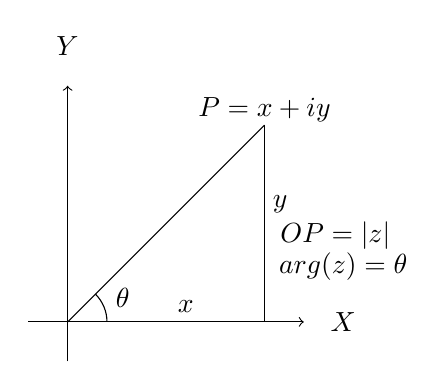
\begin{tikzpicture}
      \draw[->] (-.5,0) -- (3,0);
      \draw[->] (0,-.5) -- (0,3);
      \draw (0, 3.5) node {$Y$};
      \draw (3.5, 0) node {$X$};
      \draw (2.5,0) -- (2.5,2.5);
      \draw (0,0) -- (2.5, 2.5);
      \draw (.5,0) arc(0:45:.5);
      \draw (.7,.3) node{$\theta$};
      \draw (1.5, 0.2) node {$x$};
      \draw (2.7, 1.5) node {$y$};
      \draw (3.4, 1.1) node {$OP=|z|$};
      \draw (3.5, 0.7) node {$arg(z)=\theta$};
      \draw (2.5, 2.7) node{$P=x+iy$};
    \end{tikzpicture}
    \caption{Complex number in argand plane or complex plane}
  \end{center}
\end{figure}

In the diagram, $\theta$ is known as the \textit{argument} of $z$. This is nothing but angle made with positive direction
(i.e. counter-clockwise) of real axis. Now, this argument is not unique. If $\theta$ is an argument of a complex number $z$ then,
$2n\pi + theta$, where $n\in I$, where I is the set of integers. The value of argument for which $-\pi<\theta\leq \pi$ is called
the \textit{principal value} of \textit{argument} or \textit{principal argument}.

\subsection{Different Arguments of a Complex Number}
In the diagram, the argument is given as $\arg(z) = \tan^{-1}\left(\frac{y}{x}\right)$, this value is for when $z$ in first
quadrant. When $z$ will lie in second, third and fourth quadrants the arguments will be
$$\arg(z) = \pi - \tan^{-1}\left(\frac{y}{|z|}\right), arg(z)= -\pi + \tan^{-1}\left(\frac{|y|}{|z|}\right)\text{~and~} arg(z) =
-\tan^P{-1}\left(\frac{|y|}{x}\right)$$
respecticely.

\subsection{Polar Form of a Complex Number}
If $z$ is a non-zero complex number, then we can write $z = r(\cos\theta + i\sin\theta)$, where $r = |z|$ and $\theta = arg(z)$.

In this case, $z$ is also given by $z = r[\cos(2n\pi  \theta) + i\sin(2n\pi + \theta)]$, where $n\in I$.

\subsubsection{Euler's Formula}
The complex number $\cos\theta + i\sin\theta$ is denoted by $e^{i\theta}$ or $c$ is $\theta$, where $c$ is the complex number.

\subsection{Important Results Involving Arguments}
If $z, z_1$ and $z_2$ are complex numbers, then

\begin{enumerate}
\item $arg(\overline{(z)}) = -arg(z)$. This can be easily proven as if $z = x + iy$, then $\overline{z} = x - iy$ i.e. sign of
  argument will get a -ve sign as $y$ gets one.
\item $arg(z_1z_2) = arg(z_1)  + arg(z_2) + 2n\pi$, where
  $$n = \begin{cases}
   0 \text{~if~} & -\pi<arg(z_1)+arg(z_2)\leq-\pi\\
   1 \text{~if~} & -2\pi<arg(z_1)+arg(z_2)\leq-\pi\\
   -1 \text{~if~} & -\pi<arg(z_1)+arg(z_2)\leq2\pi\end{cases}$$
 \item Similarly, $arg(z_1\overline{z_2}) = arg(z_1) - arg(z_2)$.
 \item $|z_1 + z_2| = |z_2 - z_2| \Leftrightarrow arg(z_1) - arg(z_2) = \pi/2$.
 \item $|z_1 + z_2| = |z_1| + |z_2| \Leftrightarrow arg(z_1) = arg(z_2)$.
 \item $|z_1 + z_2|^2 = r_1^2 + r_2^2 + 2r_1r_2\cos(\theta_1 - \theta_2)$.
 \item $|z_1 - z_2|^2 = r_1^2 +r_2^2 + 2r_1r_2\cos(\theta_1 + \theta_2)$.
\end{enumerate}

\section{Vector Representation}
Complex numbers can also be represented as vectors. Length of the vector is nothing but modulus of complex number and argument is
the angle which the vector makes with read axis. It is denoted as $\overrightarrow{OP}$, where $OP$ represents the vector of the
complex number $z$.

\section{Algebraic Operation's Representation}
Let $z_1 = x_1 + iy_1$ and $z_2 = x_2 + iy_2$ be two complex numbers, which are represented by two point $P_1$ and $P_2$ in the
following diagrams.

\subsection{Addition}
Now, as we know that $z_1 + z_2 = (x_1 + x_2) + i(y_1 + y_2)$. Let us see how it looks using geometrically:
\begin{figure}[h]
  \begin{center}
    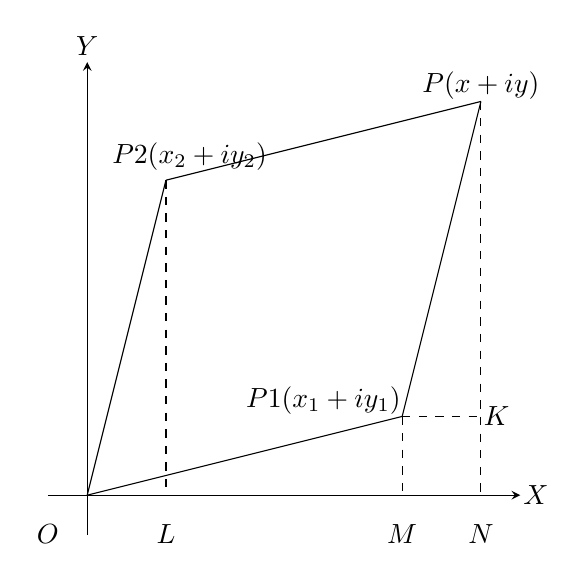
\begin{tikzpicture}
      \draw[->, >=stealth] (-.5,0) -- (5.5,0);
      \draw[->, >=stealth] (0,-.5) -- (0,5.5);
      \draw (5.7, 0) node {$X$};
      \draw (0,5.7) node {$Y$};
      \draw (0,0) -- (4,1);
      \draw (0,0) -- (1,4);
      \draw (1,4) -- (5,5);
      \draw (4,1) -- (5,5);
      \draw[dashed] (4,1) -- (4,0);
      \draw[dashed] (1,4) -- (1,0);
      \draw[dashed] (5,5) -- (5,0);
      \draw[dashed] (4,1) -- (5,1);
      \draw (-.5,-.5) node {$O$};
      \draw (1,-.5) node {$L$};
      \draw (4,-.5) node {$M$};
      \draw (5,-.5) node {$N$};
      \draw (5.2,1) node {$K$};
      \draw (3, 1.2) node {$P1(x_1+iy_1)$};
      \draw (1.3, 4.3) node {$P2(x_2+iy_2)$};
      \draw (5, 5.2) node {$P(x+iy)$};
    \end{tikzpicture}
    \caption{Complex numbers addition}
  \end{center}
\end{figure}
Clearly, $z = z_1 + z_2 = x_1 + x_2 + i(y_1 + y_2)$. Let $P_1M, P_2L$ and $PN$ be parallel to the $y$-axis; $P_1K$ be parallet to
the $x$-axis. This implied that triangle $OP_2L$ and $PP_1K$ are congruent.

We have $P_1K = OL = x_1$ and $P_2L = PK = y_1$

Thus, $ON = OM + MN = OL + P_1K = x_1 + x_2$ and $PN = PK + KN = P_2L + P_1M = y_2 + y_1$

So we can say that coordinates of $P$ are $(x_1 + x_2, y_1 + y_2)$ which represents the complex number $z.$

We also see that this obeys vector addition i.e. $OP_1 + OP_2 = OP_1 + P_1P = OP$

\subsection{Subtraction}
\begin{figure}[h]
  \begin{center}
    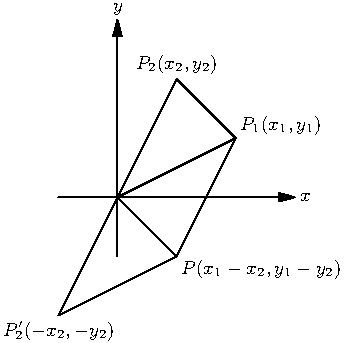
\includegraphics{complex-numbers-subtraction}
    \caption{Complex numbers subtraction}
  \end{center}
\end{figure}
We first represent $-z_2$ by $P_2'$ so that  $P_2P_2'$ is bisected at $O.$ Complete the parallelogram $OP_1PP_2'.$ Then it can be
easily seen that $P$  representd the difference $z_1 - z_2.$

As $OP_1PP_2'$ is a parallelogram so $P_1P = OP_2'.$ Using vetor notation, we have, $z_1 - z_2 = OP_1 - OP_2 = OP_1 + OP_2' = OP_1 + P_1P = P_2P1$

It follows that the complex number $z_1 - z_2$ is represented by the vector $P_1P_2,$ where points $P_1$ and $P_2$ represent the
complex numbers $z_1$ and $z_2$ respectively.

It should be noted that $arg(z_1 - z_2)$ is the angle through which $OX$ must be rotated in the anticlockwise direction to make it
parallel with $P_1P_2.$

\subsection{Multiplication}
\begin{figure}[H]
  \begin{center}
    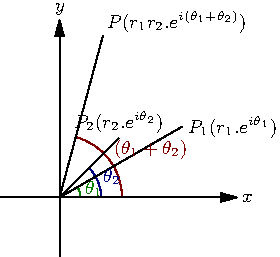
\includegraphics{complex-numbers-multiplication}
    \caption{Complex numbers multiplication}
  \end{center}
\end{figure}
For multiplication it is convenient to use Euler's formula of complex numbers.

Let $z_1 = r_1e^{i\theta_1}$ and $z_2 = r_2e^{i\theta_2},$ then clealry, $z_1z_2 = r_1r_2e^{i(\theta_1 + \theta_2)}$

\part{Solutions}
\chapter{Logarithm}
\begin{enumerate}
\item $\log_{\sqrt{8}}x = \frac{10}{3} \Rightarrow \log_{2^{\tfrac{3}{2}}}x = \frac{10}{3}\Rightarrow \frac{2}{3}\log_2x = \frac{10}{3}$

  $\Rightarrow \log_2x = 5 \Rightarrow x = 2^5 = 32.$
\item L.H.S. $= \log_ba.\log_cb\log_ac = \frac{\log a}{\log b}.\frac{\log b}{\log c}.\frac{\log c}{\log a} = 1 =$ R.H.S.
\item L.H.S. $= \log_3\log_2\log_{\sqrt{5}}(\sqrt{5})^8 = \log_3\log_28 = \log_33 = 1 =$ R.H.S.
\item Given $a^2 + b^2 = 23ab \Rightarrow (a + b)^2 = 25ab \Rightarrow \frac{a + b}{5} = \sqrt{ab}$

  Taking $\log$ of both sides, we get

  $\log\frac{a + b}{5} = \frac{1}{2}(\log a + \log b)$.
\item L.H.S. $= 7\log\frac{16}{15} + 5\log\frac{25}{24} + 3\log\frac{81}{80} = \log 2$

  $= 7[\log 2^4 - \log 3.5] + 5[\log 5^2 - \log 2^3.3] + 3[\log 3^4 - \log 2^4.5]$

  $= 7[4\log 2 - \log 3 - \log 5] + 5[2\log 5 - 3\log 2 - \log 3] + 3[4\log 3 - 4\log 2 - \log 5]$

  $= \log 2 =$ R.H.S.
\item L.H.S. $= \log\tan1^\circ + \log\tan2^\circ + \ldots + \log\tan89^\circ$

  $= (\log\tan1^\circ + \log\tan89^\circ) + (\log\tan2^\circ + \log\tan88^\circ) + \cdots + \log\tan45^\circ$

  $=(\log\tan1^\circ\cot1^\circ) + (\log\tan2^\circ\cot2^\circ) + \cdots + \log\tan45^\circ [\because \tan(90^\circ - \theta) =
  \cot\theta]$

  $= \log 1 + \log 1 + \cdots + \log 1 = 0 [\because \tan\theta\cot\theta = 1]$
\item Given $\log_9\tan\frac{\pi}{6} = \log_9\frac{1}{\sqrt{3}} = -\log_9\sqrt{3} = -\log_99^{1/4} = -\frac{1}{4}$.
\item Given $\frac{\log_{a^2}b}{\log_{\sqrt{a}}b^2} = \frac{\frac{1}{2}\log_ab}{2.2\log_ab} = \frac{1}{8}$.
\item Given $\log_{\sqrt{5}}.008 = 2\log_6\frac{8}{1000} = 2[\log_58 - \log_51000] = 2[\log_58 - \log 8.125]$

  $= 2[\log_58 - \log_68 - \log_5125] = -2.\log_55^3 = -6$.
\item Given $\log_{2\sqrt{3}}144 = \log_{2\sqrt{3}}(2\sqrt{3})^4 = 4$.
\item L.H.S. $= \log_3\log_2\log_{\sqrt{3}}81 = \log_3\log_2\log_{\sqrt{3}}(\sqrt{3})^8 = \log_3\log_28 = \log_33 = 1 =$ R.H.S.
\item L.H.S. $= \log_ax\log_by = \frac{\log x}{\log a}.\frac{\log y}{\log b} = \frac{\log x}{\log b}.\frac{\log y}{\log a}$

  $= \log_bx\log_ay =$ R.H.S.
\item L.H.S. $= \log_2\log_2\log_216 = \log_2\log_2\log_22^4 = \log_2\log_24 = \log_22 = 1 =$ R.H.S.
\item R.H.S. $= \log_bx\log_cb\ldots\log_nm\log_an = \frac{\log x}{\log b}.\frac{\log b}{\log c}\cdots\frac{\log m}{\log
  n}.\frac{\log n}{\log a}$

  $= \frac{\log x}{\log a} = \log_ax =$ L.H.S.
\item Let $10^x\log_{10}a = z$.

  Taking $\log$ of both sides, we get

  $x\log_{10}a = \log z \Rightarrow \log_{10}a^x = \log z \Rightarrow z = a^x$.
\item Given $a^2 + b^2 = 7ab \Rightarrow a^2 + b^2 + 2ab = (a + b)^2 = 9ab$

  $\Rightarrow \left(\frac{a + b}{3}\right)^2 = ab \Rightarrow \frac{a + b}{3} = \sqrt{ab} = (ab)^{1/2}$

  Taking $\log$ of both sides,

  $\log \frac{a + b}{3} = \frac{1}{2}(\log a + \log b)$.
\item L.H.S. $= \frac{\log_a\log_ba}{\log_b\log_ab}$

  Let $\log_ba = z$, then L.H.S. $= \frac{\log_az}{\log_b\tfrac{1}{z}} = -\frac{\log_az}{\log_bz} = -\frac{\log z}{\log a}.\frac{\log z}{\log b}$

  $= - \frac{\log b}{\log a} = -\log_ab =$ R.H.S.
\item L.H.S. $= \log(1 + 2 + 3) = \log 6 = \log(1.2.3) = \log 1 + \log 2 + \log 3 =$ R.H.S.
\item L.H.S. $= 2\log(1 + 2 + 4 + 7 + 14) = 2\log 28 = \log 784$

  $= \log(1.2.4.7.14) = \log 1 + \log 2 + \log 4 + \log 7 + \log 14 =$ R.H.S.
\item L.H.S. $= \log 2 + 16\log\frac{16}{15} + 12\log\frac{25}{24} + 7\log\frac{81}{80}$

  $= \log 2 + 16[\log 2^4 - \log 3 - \log 5] + 12[\log 5^2 - \log 2^3 - \log 3] + 7[\log 3^4 - \log 2^4 - \log 5]$

  $= \log 2 + 16[4\log 2 - \log 3 - \log 5] + 12[2\log 5 - 3\log 2 - \log 3] + 7[4\log 3 - 4\log 2 - \log 5]$

  $= \log 2[1 + 64 - 36 - 28] + \log 3[28 - 16 -1 12] + \log 5[24 - 7 - 15]$

  $= \log 2 + \log 5 = \log 10 = 1$ [$\because$ default base of $\log$ is $10$.]
\item Given $\frac{\log_911}{\log_513}\div\frac{\log_311}{\log_{\sqrt{5}}13} =
  \frac{\log_{3^2}11}{\log_513}.\frac{\log_{5^{\tfrac{1}{2}}}11}{\log_3 11}$

  $= \frac{\tfrac{1}{2}\log_311}{\log_513}.\frac{2\log_513}{\log_311} = 1$.
\item Given, $3^{\sqrt{\log_32}} - 2^{\sqrt{\log_23}}$

  Taking $\log$ with base $10$,

  $\sqrt{\log_32}\log 3 - \sqrt{\log_23}\log 2 = \sqrt{\frac{\log 2}{\log 2}(\log 3)^2} - \sqrt{\frac{\log 3}{\log 2}(\log 2)^2}$

  $= \sqrt{\log 2\log 3} - \sqrt{\log 3\log 2} = 0$.
\item Given $\log_{10}343 = 2.5353 \Rightarrow \log_{10}7^3 = 2.5353 \Rightarrow \log_{10}7 = o.8451$

  For $7^n > 10^5 \Rightarrow n\log_{10}7 > 5 \Rightarrow n > \frac{5}{0.8451}$

  Thus, least such integer is $6$.
\item Since $a, b, c$ are in G.P., we can write $b^2 = ac$

  Taking $\log$ of both sides, we get

  $2\log b = \log a + \log c \Rightarrow \log a, \log b, \log c$ are in A.P.

  i.e. $\frac{1}{\log a}, \frac{1}{\log b}, \frac{1}{\log c}$ are in H.P.

  Multiplying each term with $\log x$,

  $\frac{\log x}{\log a}, \frac{\log x}{\log b}, \frac{\log x}{\log c}$ are in H.P.

  $\log_ax, \log_bx, \log_cx$ are in H.P.
\item R.H.S. $= 3\log2 + \log\sin x + \log\cos x + \log\cos2x + \log\cos4x$

  $= 2\log 2 + (\log 2.\sin x\cos x) + \log\cos2x + \log\cos4x$

  $= 2\log 2 + \log\sin2x + \log\cos2x + \log\cos4x = \log 2 + (\log 2.\sin2x\cos2x) + \log\cos4x$

  $= \log 2 + \log\sin4x + \cos4x = \log 2.\sin4x\cos4x$

  $= \log\sin8x =$ L.H.S.
\item We have to prove that $xyz + 1 = 2yz \Rightarrow x + \frac{1}{yz} = 2$

  L.H.S. $= x + \frac{1}{yz}$, substituting the values of $x, y$ and $z$,

  $\log_{2a}a + \frac{1}{\log_{3a}2a\log_{4a}3a} = \frac{\log a}{\log 2a} + \frac{\log 3a.\log 4a}{\log 2a.\log 3a}$

  $= \frac{\log a + \log 4a}{\log 2a} = \frac{\log(2a)^2}{\log 2a} = 2 =$ R.H.S.
\item We have to prove that $\log_{c + b}a + \log_{c - b}a = 2\log_{c + a}a\log_{c - b}a$

  Dividing both sides by $\log_{c + b}a\log_{c - b}a$,

  $\frac{1}{\log_{c - b}a} + \frac{1}{\log_{c + b}\log a} = 2$

  $\Rightarrow \log_a(c - b) + \log_a(c + b) = 2$

  $\Rightarrow \log_a(c^2 - b^2) = 2\Rightarrow c^2 = a^2 + b^2$

  which is true because $c$ is hypotenuse and $a$ and $b$ are sides of a right-angle triangle.
\item Let $\frac{\log x}{y - z} = \frac{\log y}{z - x} = \frac{\log z}{x - y} = k$

  $\log x = k(y - z), \log y = k(z - x), \log z = k(x - y)$

  $\Rightarrow x\log x + y\log y + z\log z = k(xy - zx + yz - xy + zx - yz) = 0$

  $\Rightarrow \log x^x + \log y^y + \log z^z = \log x^xy^yz^z = 0$

  $\Rightarrow x^xy^yz^z = 1$.
\item Given $\frac{yz\log(yz)}{y + z} = \frac{zx\log(zx)}{z + x} = \frac{xy\log(xy)}{x + y}$

  Dividing by $xyz, \frac{\log(yz)}{x(y + z)} = \frac{\log(zx)}{y(z + x)} = \frac{\log(xy)}{z(x + y)} = k$ (let)

  $\log y + \log z = k(xy + yz), \log z + \log x = k(yz + xy), \log x + \log y = k(yz + zx)$

  $\Rightarrow x\log x = kyz \Rightarrow x\log x = kxyz = y\log y = z\log z$

  $\Rightarrow x^x = y^y = z^z$.
\item We have to prove that $(yz)^{\log y - \log z}(zx)^{\log z - \log x}(xy)^{\log x - \log y} = 1$

  Taking $\log$ of both sides,

  $\Rightarrow (\log y - \log z)(\log y + \log z) + (\log z - \log x)(\log z + \log x) + (\log x - \log y)(\log x + \log y) = 0$

  $\Rightarrow (\log y)^2 - (\log z)^2 + (\log z)^2 - (\log x)^2 + (\log x)^2 - (\log y)^2 = 0$

  $\Rightarrow 0 = 0$.
\item L.H.S $= \log_N2 + \log_n3 + \cdots + \log_n1988$

  $= \log_N(2.3.4.\ldots1988) = \log_N1988! = \frac{1}{\log_{1988!}N} =$ R.H.S.
\item L.H.S. $= \log(1 + x) + \log(1 + x^2) + \log(1 + x^4)\ldots~{\rm to}~\infty$

  $= \log(1 + x + x^2 + \ldots~{\rm to}~\infty)$

  $= \log\frac{1}{1 - x}[\because 0 < x < 1]$ (from the formula for the sum of an infinite G.P.)

  $= -\log(1 - x) =$ R.H.S.
\item Let $S_n = \frac{1}{\log_2a} + \frac{1}{\log_4a} + \cdots$ up to $n$ terms

  $S_n = \log_a2 + \log_a4 + \log_a8 + \cdots$ up to $n$ terms

  $S_n = (1 + 2 + 3 + \cdots + n)\log_a2 = \frac{n(n + 1)}{2}\log_a2$.
\item L.H.S. $= \frac{1}{x + 1} + \frac{1}{y + 1} + \frac{1}{z + 1}$

  $= \frac{1}{\log_410 + \log_44} + \frac{1}{\log_220 + \log_220} + \frac{1}{\log_58 + \log_55}$

  $= \frac{1}{\log_440} + \frac{1}{\log_240} + \frac{1}{\log_540}$

  $= \log_{40}4 + \log_{40}2 + \log_{40}5 = \log_{40}(4.2.5) = \log_{40}40 = 1 =$ R.H.S.
\item L.H.S. $= \frac{1}{\log_abc + 1} + \frac{1}{\log_bca + 1} + \frac{1}{\log_cab + 1}$

  $= \frac{1}{\log_abc + \log_aa} + \frac{1}{\log_bca + \log_bb} + \frac{1}{\log_cab + \log_cc}$

  $= \frac{1}{\log_aabc} + \frac{1}{\log_babc} + \frac{1}{\log_cabc}$

  $= \log_{abc}a + \log_{abc}b + \log_{abc}c = \log_{abc}abc = 1 =$ R.H.S.
\item Given, $\frac{1}{1 + \log_ba + \log_bc} + \frac{1}{1 + \log_ca + \log_cb} + \frac{1}{1 + \log_ab + \log_ac} = 1$

  L.H.S. $= \frac{1}{\log_ba + \log_ba + \log_bc} + \frac{1}{log_cc + \log_ca + \log_cb} + \frac{1}{\log_aa + \log_ab + \log_ac}$

  $= \frac{1}{\log_babc} + \frac{1}{\log_cabc} + \frac{1}{\log_aabc}$

  Like previous problem the above expression will evaluate to $1$.
\item We have to prove that $x^{\log y - \log z}y^{\log z - \log x}z^{\log x - \log y} = 1$

  Taking $\log$ of both sides,

  $(\log y - \log z)\log x + (\log z - \log x)\log y + (\log x - \log y)\log z = 0$

  $\Rightarrow \log y\log z - \log z\log x + \log z\log y - \log x\log y + \log x\log z - \log y\log z = 0$

  $\Rightarrow 0 = 0$.
\item Let $\frac{\log a}{y - z} = \frac{\log b}{z - x} = \frac{\log c}{x - y} = k$

  $\Rightarrow x\log a = k(xy - zx), y\log b = k(yz - xy), z\log c = k(zx - yz)$

  Adding all,

  $x\log a + y\log b + z\log c = k(xy - zx + yz - xy + zx - yz) = 0$

  $\log a^xb^yx^z = 0\Rightarrow a^xb^yc^z = 1$
\item Let $\frac{x(y + z - x)}{\log x} = \frac{y(z + x - y)}{\log y} = \frac{z(x + y - z)}{\log z} = \frac{1}{k}$

  $\Rightarrow \log x = kx(y + z - x), \log y = ky(z + x - y), \log z = kz(x + y - z)$

  Let $y^zz^y = z^xz^z = x^yy^x$

  Taking $\log$, we have

  $z\log y + y\log z = x\log z + z\log x = y\log x + x\log y$

  $\Rightarrow zky(z + x - y) + ykz(x + y - z) = xkz(x + y - z) + zkx(y + z - x) = ykx(y + z - x) + xky(x + z - y)$

  $\Rightarrow yz^2 + xyz - y^2z + xyz + y^2 - z^2y = x^2z + xyz - xz^2 + xyz + xz^2 - x^2z = xy^2 + xyz - x^2y + x^2y + xyz -
  xy^2$

  $\Rightarrow 2xyz = 2xyz = 2xyz$.
\item Let $\frac{\log a}{b - c} = \frac{\log b}{c - a} = \frac{\log c}{a - b} = k$

  $\Rightarrow \log a = k(b - c), \log b = k(c - a), \log c = k(a - b)$

  $\Rightarrow (b + c)\log a = k(b^2 - c^2), (c + a)\log b = k(c^2 - a^2), (a + b)\log c = k(a^2 - b^2)$

  Adding all, $\log a^{b + c} + \log b^{c + a} + \log c^{a + b} = 0$

  $\Rightarrow a^{b + c}b^{c + a}c^{a + b} = 1$.
\item Let $\frac{\log x}{q - r} = \frac{\log y}{r - p} = \frac{\log z}{p - q} = k$

  $\Rightarrow \log x = k(q - r), \log y = k(r - p), \log z = k(p - q)$

  $\Rightarrow (q + r)\log x = k(q^2 - r^2), (r + p)\log y = k(r^2 - p^2), (p + q)\log z = k(p^2 - q^2)$

  Adding all $\log x^{q + r} + \log y^{r + p} + \log z^{p + q} = 0$

  $\Rightarrow x^{q + r}y^{r + p}z^{p + q} = 1$.

  Similarly, $p\log x = kp(q - r), q\log y = kq(r - p), r\log z = kr(p - q)$

  Adding all, $\log x^p + \log y^q + \log z^r = 0 \Rightarrow x^py^qz^r = 1$.
\item Given $y = a^{\tfrac{1}{1 - \log_ax}}$ and $z = a^{\tfrac{1}{1 - \log_ay}}$

  $\therefore z = a^{\tfrac{1}{1 - \log_aa^{\left(\tfrac{1}{1 - \log_ax}\right)}}} = a^{\tfrac{1}{1 - \tfrac{1}{1 - \log_ax}}}$

  Taking $\log$ of both sides with base $a$,

  $\log_az = \frac{1}{1 - \tfrac{1}{1 - \log_ax}} = \frac{1 - \log_ax}{-\log_ax} = 1 - \frac{1}{\log_ax}$

  $\Rightarrow x = a^{\tfrac{1}{1 - \log_az}}$.
\item Given $f(y) = e^{f(z)}$ and $z = e^{f(x)}$, where $f(x) = \frac{1}{1 - \log_ex}$

  $f(y) = e^{\tfrac{1}{1 - \log_ez}} = e^{\tfrac{1}{1 - \log_ee^{\tfrac{1}{1 - \log_ex}}}} = e^{\tfrac{1}{1 - \tfrac{1}{1 -
      \log_ex}}}$

  Following like above exercie $x = e^{f(y)}$.
\item L.H.S. $= \frac{1}{\log_2n} + \frac{1}{\log_3n} + \frac{1}{\log_4n} + \cdots + \frac{1}{\log_{43}n}$

  $= \log_n2 + \log_n3 + \log_n4 + \cdots + \log_n43 = \log_n(2.3.4\ldots 43)$

  $= \log_n43! = \frac{1}{\log_{43!}n} =$ R.H.S.
\item L.H.S. $= (1 + 2 + 3 + \cdots + n).2\log a = \frac{n(n + 1)}{2}.2\log a = n(n + 1)\log a =$ R.H.S.
\item We will use of the fact that positive characteristics of $n$ of a logarithmm means that there $n + 1$ digits in the number.

  Let $\log y = 12\log 12 = 12\log(2.2.3) = 12[2\times0.301 + 0.477] = 12.96$.

  Thus, number of digits is $13$.
\item We can use the fact that the number of positive integers having base $b$ and characteristics $n$ is $b^{n + 1} - b^n$.

  Thus, number of integer with base $3$ and characteristics $2$ is $3^3 - 3^3 = 18$.
\item Let $y = (0.0504)^{10} \Rightarrow \log_{10}y = 10\log_{10}(0.504) = 10\log_{10}(504\times10^-4)$

  $= -10\log_{10}[-4 + \log(2^3.3^2.7)] = -12.98$.

  Thus, characteristics is $-13$. Therefore, number of zeros after decimal and first significant digit is $12$.
\item Let $x = 72^{15} \therefore \log_{10}x = 15\log_{10}72 = 15\log_{10}(2^3\times3^2) = 15[3\log_{10}2 + 2\log_{10}3]$

  $i = 15[3\times0.301 + 2\times0.477] = 15[0.903 + 0.954] = 15\times1.857 = 27.855$

  So the characteristics is $27$ and hence the number of digits will be $28$.
\item Given $b = 5, n = 2$, therefore the number of integers will be $5^3 - 5^2 - 100$.
\item Let $x = 3^{15}\times 2^{10} \therefore \log_{10}x = 15\log_{10}3 + 10\log_{10}2$

  $= 15\times0.477 + 10\times 0.301 = 10.165$.

  So no. of digits will be $11$.
\item Let $x = 6^{20} \therefore \log_{10}x = 20\log_{10}(2\times3) = 20[\log_{10}2 + \log_{10}3]$

  $= 20[0.301 + 0.477] = 15.56$.

  So no. of digits will be $16$.
\item Let $x = 5^{25} \therefore \log_{10}x = 25\log_{10}\frac{10}{2}= 25[1 - \log_{10}2]$

  $= 25\times 0.699 = 17.475$

  So no. of digits will be $18$.
\item Given $\log_a[1 + \log_b\{1 + \log_c(1 + \log_px)\}] = 0$

  $\Rightarrow 1 + \log_b\{1 + \log_c(1 + \log_px)\} = 1$

  $\Rightarrow \log_b\{1 + \log_c(1 + \log_px)\} = 0$

  $\Rightarrow 1 + \log_c(1 + \log_px) = 1$

  $\Rightarrow \log_c(1 + \log_px) = 0$

  $\Rightarrow 1 + \log_px = 1$

  $\Rightarrow \log_px = 0 \Rightarrow x = 1$
\item Given $\log_7\log_5(\sqrt{x + 5} + \sqrt{x}) = 0 \Rightarrow \log_5(\sqrt{x + 5} + \sqrt{x}) = 1$

  $\Rightarrow \sqrt{x + 5} + \sqrt{x} = 5 \Rightarrow \sqrt{x + 5} = 5 - \sqrt{x}$

  Squaring both sides,

  $x + 5 = 25 + x - 10\sqrt{x}\Rightarrow \sqrt{x} = 2\Rightarrow x = 4$.
\item $\log_2x + \log_4(x + 2) = 2 \Rightarrow \log_2x + \frac{1}{2}\log_2(x + 2) = 2$

  $\Rightarrow 2\log_2x + \log_2(x + 2) = 4 \Rightarrow \log_2x^2(x + 3) = 4$

  $\Rightarrow x^2(x + 2) = 16 \Rightarrow x = 2$
\item $\log_{(x + 2)}x + \log_x(x + 2) = \frac{5}{2} \Rightarrow \frac{1}{\log_x(x + 2)} + \log_x(x + 2) = \frac{5}{2}$

  Let $z = \log_x(x + 2) \Rightarrow \frac{1}{z} + z = \frac{5}{2}$

  $2z^2 + 2 - 5z = 0 \Rightarrow z = 2, \frac{1}{2}$

  $\Rightarrow \log_x(x + 2) = 2, \frac{1}{2}$

  $\Rightarrow x + 2 = 2^2, x + 2 = \sqrt{x}$

  $x = 2, x^2 - 4x + 4 = 0 \Rightarrow x = \frac{3\pm\sqrt{-7}}{2}$

  However, $x$ cannot be a complex number. $\therefore x = 2$.
\item $\frac{\log(x + 1)}{\log x} = 2\Rightarrow \log_x(x + 1) = 2 \Rightarrow x + 1 = x^2$

  $\Rightarrow x = \frac{1\pm \sqrt{5}}{2}$

  $\because x > 0, x = \frac{1 + \sqrt{5}}{2}$.
\item $2\log_xa + \log_{ax}a + 3\log_{a^2x}a = 0 \Rightarrow \frac{2}{\log_ax} + \frac{1}{\log_aax} + \frac{1}{\log_aa^2x} = 0$

  $\Rightarrow \frac{2}{\log_ax} + \frac{1}{\log_aa + \log_ax} + \frac{1}{\log_aa^2 + \log_ax} = 0$

  $\Rightarrow \frac{2}{\log_ax} + \frac{1}{1 + \log_ax} + \frac{1}{2 + \log_ax} = 0$

  Substituting $\log_ax = z, \frac{2}{z} + \frac{1}{1 + z} + \frac{1}{2 + z} = 0$

  $\Rightarrow 6z^2 + 11z + 4 = 0 \Rightarrow z = -\frac{1}{2}, -\frac{4}{3}$

  $\therefore x = a^{-\tfrac{1}{2}}, a^{-\tfrac{4}{3}}$.
\item $x + \log_{10}(1 + 2^2) = x\log_{10}5 + \log_{10}6$

  $\Rightarrow \log_{10}10^x + \log_{10}(1 + 2^x) = \log_{10}5^x + \log_{10}6$

  $\Rightarrow \log_{10}10^x(1 + x^x) = \log_{10}(5^x.6)$

  $\Rightarrow 2^x(1 + 2^x) = 2.3 \Rightarrow 2^x = 2, 1 + 2^x = 3 \Rightarrow x = 1$.
\item $x^{\tfrac{3}{4}(\log_2x)^2 + \log_2x - \tfrac{5}{4}} = \sqrt{2}$

  Taking $\log_2$ of both sides,

  $\left[\frac{3}{4}(\log_2x)^2 + \log_2x - \frac{5}{4}\right]\log_2x = \frac{1}{2}\log_22$

  $\left[\frac{3}{4}(\log_2x)^2 + \log_2x - \frac{5}{4}\right]\log_2x = \frac{1}{2}$

  Let $\log_2x = z, \Rightarrow \left(\frac{3}{4}z^2 + z - \frac{5}{4}\right)z = \frac{1}{2}$

  Solving this qubic equation yields $x = 2, \frac{1}{4}, \frac{1}{\sqrt[3]{2}}$.
\item Given $(x^2 + 6)^{\log_3x} = (5x)^{\log_3x}$

  $\log_3x$ has a possible value of $0$, in that case $x = 1$

  If $\log_3x\neq 0, \Rightarrow x^2 + 6 = 5x \Rightarrow x = 2, 3$.
\item Given, $(3 + 2\sqrt{2})^{x^2 - 6x + 9} + (3 - 2\sqrt{2})^{x^2 - 6x + 9} = 6$

  We observe that $3 + 2\sqrt{2} = \frac{1}{3 - 2\sqrt{2}}$, thus, given equation becomes

  $(3 + 2\sqrt{2})^{x^2 - 6x + 9} + (3 + 2\sqrt{2})^{-(x^2 - 6x + 9)} = 6$

  Let $z = (3 + 2\sqrt{2})^{x^2 - 6x + 9}\Rightarrow z + \frac{1}{z} = 6 \Rightarrow z = 3\pm2\sqrt{2}$

  Thus, $x^2 - 6x + 9 = \pm 1 \Rightarrow x = 2, 4$ because other roots are irrational.
\item Given, $\log_8\left(\frac{8}{x^2}\right)\div(\log_8x)^2 = 3$

  $\Rightarrow \log_88 - \log_8x^2 = 3(\log_8x)^2 \Rightarrow 1 - 2\log_8x = 3(\log_8x)^2$

  Let $z = \log_8x\Rightarrow 1 - 2z = 3z^2 \Rightarrow z = -1, \frac{1}{3}\Rightarrow x = 2, \frac{1}{8}$.
\item Given, $\sqrt{\log_2(x)^4} + 4\log_4\sqrt{\tfrac{2}{x}} = 2$

  $\Rightarrow \sqrt{\log_2(x)^4} + 2\log_2\sqrt{\tfrac{2}{x}} = 2$

  $\Rightarrow \sqrt{4\log_2x} + \log_2\tfrac{2}{x} = 2$

  $\Rightarrow \sqrt{4\log_2x} + 1 - \log_2x = 2 \Rightarrow \sqrt{4\log_2x} = 1 + \log_2x$

  Squaring, $4\log_2x = 1 + 2\log_2x + (\log_2x)^2 \Rightarrow (\log_2x - 1)^2 = 0$

  $\Rightarrow \log_2x = 1 \Rightarrow x = 2$.
\item Given, $2\log_{10}x - \log_x0.01 = 5 \Rightarrow 2\log_{10}x - \log_x(10)^{-2} = 5$

  $\Rightarrow 2\log_{10}x - \log_x(10)^{-2} = 5 \Rightarrow 2\log_{10}x + 2\log_x10 = 5$

  $\Rightarrow 2\log_{10}x + \frac{2}{\log_{10}x} = 5$

  Let $z = \log_{10}x \Rightarrow 2z + \frac{2}{z} = 5 \Rightarrow z = 2, \frac{1}{2}$

  $\Rightarrow x = 100, \sqrt{10}$.
\item Given, $\log_{\sin x}2\log_{\cos x}2 + \log_{\sin x}2 + \log_{\cos x}2 = 0$

  $\Rightarrow \log_{\sin x}2(\log_{\cos x}2 + 1) + \log_{\cos x}2 = 0$

  $\Rightarrow \frac{\ln 2}{\ln \sin x}\left(\frac{\ln 2}{\ln \cos x} + 1\right) + \frac{\ln 2}{\ln \cos x} = 0$

  $\Rightarrow \frac{1}{\ln \sin x}\left(\frac{\ln 2}{\ln \cos x} + 1\right) + \frac{1}{\ln \cos x} = 0$

  $\Rightarrow \frac{1}{\ln \sin x}\left(\frac{\ln 2}{\ln \cos x} + 1\right) = -\frac{1}{\ln \cos x}$

  $\Rightarrow \frac{1}{\ln \sin x}(\ln 2 + \ln\cos x) = -1$

  $\Rightarrow \ln(\sin2x) = 0\Rightarrow x = 2k\pi + \frac{\pi}{4}, k\in\mathbb{I}$.
\item Given, $2^{x + 3} + 2^{x+2} + 2^{x + 1} = 7^x + 7^{x - 1}$

  $\Rightarrow 2^{x + 1}(2^2 + 2 + 1) = 7^{x - 1}(7 + 1) \Rightarrow 2^{x - 2} = 7^{x - 2}$

  Taking $\log$ of both sides

  $(x - 1)\log 2 = (x - 2)(\log 7), \because 2\neq 7 \Rightarrow x = 2$.
\item Given, $\log_{\sqrt{2}\sin x}(1 + \cos x) = 2$

  $\Rightarrow 1 + \cos x = (\sqrt{2}\sin x)^2 = 2\sin^2x = 2 - 2\cos^2 x$

  $\Rightarrow 2\cos^2x + \cos x - 1 = 0 \Rightarrow \cos x = -1, \frac{1}{2}$

  $\Rightarrow x = 2n\pi,\,2n\pi + \frac{\pi}{3}, n\in I$
\item Given, $\log_{10}[98 + \sqrt{x^2 - 12x + 36}] = 2$

  $\Rightarrow 98 + \sqrt{x^2 - 12x + 36} = 10^2 = 100$

  $\Rightarrow x^2 - 12x + 36 = 4 \Rightarrow x^2 - 12x + 32 = 0$

  $\Rightarrow x = 4, 8$.
\item Given, $2^x3^{2x} - 100 = 0 \Rightarrow x\log_{10}2 + 2x\log_{10}3 = \log_{10}100 = 2$

  Substituting values for $\log_{10}2$ and $\log_{10}3$, we get

  $0.30103x + 0.95424x = 2 \Rightarrow x = 1.593$.
\item Given, $\log_x3\log_{\tfrac{x}{3}}3 + \log_{\tfrac{x}{81}}3 = 0$

  $\Rightarrow \frac{1}{\log_3x}.\frac{1}{\log_x\tfrac{x}{3}} + \frac{1}{\log_3\tfrac{x}{81}} = 0$

  $\Rightarrow \frac{1}{\log_3x}.\frac{1}{\log_3x - \log_33} + \frac{1}{\log_3x - \log_381} = 0$

  Let $z = \log_3x, \Rightarrow \frac{1}{z}.\frac{1}{z - 1} + \frac{1}{z - 4} = 0$

  $\Rightarrow z - 4 + z^2 - z = 0 \Rightarrow z^2 - 4 = 0 \Rightarrow z = \pm 2$

  $\Rightarrow x = 9, \frac{1}{9}$.
\item Given, $\log_{(2x + 3)}(6x^2 + 23x + 21) = 4 - \log_{(3x + 7)}(4x^2 + 12x + 9)$

  $\Rightarrow \log_{(2x + 3)}(2x + 3)(3x + 7) = 4 - \log_{(3x + 7)}(2x + 3)^2$

  $\Rightarrow 1 + \log_{(2x + 3)}(3x + 7) = 4 - 2\log_{(3xx + 7)}(2x + 3)$

  Let $z = \log_{(2x + 3)}(3x + 7)$,

  $\Rightarrow 1 + z = 4 - \frac{2}{z}\Rightarrow z = 1, 2 \Rightarrow x = -4, -3, -\frac{1}{4}$.

  For logarithm to be defined, $2x + 3 > 0,\,2x + 3\neq 1$ and $3x + 7 > 0,\,3x + 7 \neq 1$.

  Thus, $x = -\frac{1}{4}$ is the only valid solution.
\item Given, $\log_2(x^2 - 1) = \log_{\tfrac{1}{2}}(x - 1)$

  $\Rightarrow \log_2(x^2 - 1) = \log_{2^{-1}}(x - 1) = -\log_2(x - 1) = \log_2\frac{1}{x - 1}$

  $\Rightarrow x^2 - 1 = \frac{1}{x - 1}\Rightarrow x = 0, x^2 - x - 1 = 0$

  $\Rightarrow x = 0, \frac{1\pm\sqrt{5}}{2}$

  For logarithm to be defined $x^2 - 1 > 0$ and $x - 1 > 0$

  Thus, $x = \frac{1+\sqrt{5}}{2}$ is the only acceptable solution.
\item Given, $\log_5\left(5^{\tfrac{1}{x} + 125}\right) = \log_56 + 1 + \frac{1}{2x}$

  $\Rightarrow \log_5\left(5^{\tfrac{1}{x} + 125}\right) - \log_56 = 1 + \frac{1}{2x}$

  $\Rightarrow \log_5\left(\tfrac{5^{\tfrac{1}{x} + 125}}{6}\right) = 1 + \frac{1}{2x}$

  $\Rightarrow 5^{\tfrac{1}{x} + 125} = 30.5^{\tfrac{1}{2x}}$

  Let $z= 5^{\tfrac{1}{2x}}$

  $\Rightarrow z^2 - 30z + 125 = 0 \Rightarrow z = 5, 25 \Rightarrow x = \frac{1}{2}, \frac{1}{4}$.
\item For $\log_{100}|x + y| = \frac{1}{2} \Rightarrow (x + y)^2 = 100$

  And for $\log_{10}y - \log_{10}|x| = \log_{100}4\Rightarrow \log_{10}\frac{y}{|x|} = \log_{10}2$

  $\Rightarrow y = 2|x| \Rightarrow y^2 = 4x^2 \Rightarrow 5x^2 + 4x|x| = 100$

  When $x > 0,\, x = \frac{10}{3}$ and when $x < 0,\,x = -10$

  $\Rightarrow y = \frac{20}{3}, 20$.
\item Given, $2\log_2\log_2x + \log_{\tfrac{1}{2}}\log_2(2\sqrt{2}x) = 1$

  $\Rightarrow \log_2(\log_2x)^2 - \log_2\log_2(2\sqrt{2}x) = 1$

  $\Rightarrow \log_2\left(\frac{(\log_2)^2}{\log_2(2\sqrt{2}x)}\right) = 1$

  $\Rightarrow \frac{(\log_2x)^2}{\log_2(2\sqrt{2}x)} = 2$

  $\Rightarrow (\log_2x)^2 = \log_2(2\sqrt{2}x)^2$

  $\Rightarrow (\log_2x)^2 - 3 - 2\log_2x = 0$

  Let $z = \log_2x$, then $z^2 - 2z - 3 = 0 \Rightarrow z = -1, 3$

  $\Rightarrow x = \frac{1}{2}, 8$

  For logarithm to be defined $x > 0, 2\sqrt{2}x > 0,\log_2x > 0, \log_2(2\sqrt{2}x) > 0$.

  Thus, $x = 8$ is only acceptable solution.
\end{enumerate}

\backmatter
\chapter*{GNU Free Documentation License}
\phantomsection  % so hyperref creates bookmarks
%\label{label_fdl}

 \begin{center}

       Version 1.3, 3 November 2008


 Copyright \copyright{} 2000, 2001, 2002, 2007, 2008  Free Software Foundation, Inc.

 \bigskip

     \texttt{<http://fsf.org/>}

 \bigskip

 Everyone is permitted to copy and distribute verbatim copies
 of this license document, but changing it is not allowed.
\end{center}


\begin{center}
{\bf\large Preamble}
\end{center}

The purpose of this License is to make a manual, textbook, or other
functional and useful document ``free'' in the sense of freedom: to
assure everyone the effective freedom to copy and redistribute it,
with or without modifying it, either commercially or noncommercially.
Secondarily, this License preserves for the author and publisher a way
to get credit for their work, while not being considered responsible
for modifications made by others.

This License is a kind of ``copyleft'', which means that derivative
works of the document must themselves be free in the same sense.  It
complements the GNU General Public License, which is a copyleft
license designed for free software.

We have designed this License in order to use it for manuals for free
software, because free software needs free documentation: a free
program should come with manuals providing the same freedoms that the
software does.  But this License is not limited to software manuals;
it can be used for any textual work, regardless of subject matter or
whether it is published as a printed book.  We recommend this License
principally for works whose purpose is instruction or reference.


\begin{center}
{\Large\bf 1. APPLICABILITY AND DEFINITIONS\par}
\phantomsection
%\addcontentsline{toc}{section}{1. APPLICABILITY AND DEFINITIONS}
\end{center}

This License applies to any manual or other work, in any medium, that
contains a notice placed by the copyright holder saying it can be
distributed under the terms of this License.  Such a notice grants a
world-wide, royalty-free license, unlimited in duration, to use that
work under the conditions stated herein.  The ``\textbf{Document}'', below,
refers to any such manual or work.  Any member of the public is a
licensee, and is addressed as ``\textbf{you}''.  You accept the license if you
copy, modify or distribute the work in a way requiring permission
under copyright law.

A ``\textbf{Modified Version}'' of the Document means any work containing the
Document or a portion of it, either copied verbatim, or with
modifications and/or translated into another language.

A ``\textbf{Secondary Section}'' is a named appendix or a front-matter section of
the Document that deals exclusively with the relationship of the
publishers or authors of the Document to the Document's overall subject
(or to related matters) and contains nothing that could fall directly
within that overall subject.  (Thus, if the Document is in part a
textbook of mathematics, a Secondary Section may not explain any
mathematics.)  The relationship could be a matter of historical
connection with the subject or with related matters, or of legal,
commercial, philosophical, ethical or political position regarding
them.

The ``\textbf{Invariant Sections}'' are certain Secondary Sections whose titles
are designated, as being those of Invariant Sections, in the notice
that says that the Document is released under this License.  If a
section does not fit the above definition of Secondary then it is not
allowed to be designated as Invariant.  The Document may contain zero
Invariant Sections.  If the Document does not identify any Invariant
Sections then there are none.

The ``\textbf{Cover Texts}'' are certain short passages of text that are listed,
as Front-Cover Texts or Back-Cover Texts, in the notice that says that
the Document is released under this License.  A Front-Cover Text may
be at most 5 words, and a Back-Cover Text may be at most 25 words.

A ``\textbf{Transparent}'' copy of the Document means a machine-readable copy,
represented in a format whose specification is available to the
general public, that is suitable for revising the document
straightforwardly with generic text editors or (for images composed of
pixels) generic paint programs or (for drawings) some widely available
drawing editor, and that is suitable for input to text formatters or
for automatic translation to a variety of formats suitable for input
to text formatters.  A copy made in an otherwise Transparent file
format whose markup, or absence of markup, has been arranged to thwart
or discourage subsequent modification by readers is not Transparent.
An image format is not Transparent if used for any substantial amount
of text.  A copy that is not ``Transparent'' is called ``\textbf{Opaque}''.

Examples of suitable formats for Transparent copies include plain
ASCII without markup, Texinfo input format, LaTeX input format, SGML
or XML using a publicly available DTD, and standard-conforming simple
HTML, PostScript or PDF designed for human modification.  Examples of
transparent image formats include PNG, XCF and JPG.  Opaque formats
include proprietary formats that can be read and edited only by
proprietary word processors, SGML or XML for which the DTD and/or
processing tools are not generally available, and the
machine-generated HTML, PostScript or PDF produced by some word
processors for output purposes only.

The ``\textbf{Title Page}'' means, for a printed book, the title page itself,
plus such following pages as are needed to hold, legibly, the material
this License requires to appear in the title page.  For works in
formats which do not have any title page as such, ``Title Page'' means
the text near the most prominent appearance of the work's title,
preceding the beginning of the body of the text.

The ``\textbf{publisher}'' means any person or entity that distributes
copies of the Document to the public.

A section ``\textbf{Entitled XYZ}'' means a named subunit of the Document whose
title either is precisely XYZ or contains XYZ in parentheses following
text that translates XYZ in another language.  (Here XYZ stands for a
specific section name mentioned below, such as ``\textbf{Acknowledgements}'',
``\textbf{Dedications}'', ``\textbf{Endorsements}'', or ``\textbf{History}''.)
To ``\textbf{Preserve the Title}''
of such a section when you modify the Document means that it remains a
section ``Entitled XYZ'' according to this definition.

The Document may include Warranty Disclaimers next to the notice which
states that this License applies to the Document.  These Warranty
Disclaimers are considered to be included by reference in this
License, but only as regards disclaiming warranties: any other
implication that these Warranty Disclaimers may have is void and has
no effect on the meaning of this License.


\begin{center}
{\Large\bf 2. VERBATIM COPYING\par}
\phantomsection
%\addcontentsline{toc}{section}{2. VERBATIM COPYING}
\end{center}

You may copy and distribute the Document in any medium, either
commercially or noncommercially, provided that this License, the
copyright notices, and the license notice saying this License applies
to the Document are reproduced in all copies, and that you add no other
conditions whatsoever to those of this License.  You may not use
technical measures to obstruct or control the reading or further
copying of the copies you make or distribute.  However, you may accept
compensation in exchange for copies.  If you distribute a large enough
number of copies you must also follow the conditions in section~3.

You may also lend copies, under the same conditions stated above, and
you may publicly display copies.


\begin{center}
{\Large\bf 3. COPYING IN QUANTITY\par}
\phantomsection
%\addcontentsline{toc}{section}{3. COPYING IN QUANTITY}
\end{center}


If you publish printed copies (or copies in media that commonly have
printed covers) of the Document, numbering more than 100, and the
Document's license notice requires Cover Texts, you must enclose the
copies in covers that carry, clearly and legibly, all these Cover
Texts: Front-Cover Texts on the front cover, and Back-Cover Texts on
the back cover.  Both covers must also clearly and legibly identify
you as the publisher of these copies.  The front cover must present
the full title with all words of the title equally prominent and
visible.  You may add other material on the covers in addition.
Copying with changes limited to the covers, as long as they preserve
the title of the Document and satisfy these conditions, can be treated
as verbatim copying in other respects.

If the required texts for either cover are too voluminous to fit
legibly, you should put the first ones listed (as many as fit
reasonably) on the actual cover, and continue the rest onto adjacent
pages.

If you publish or distribute Opaque copies of the Document numbering
more than 100, you must either include a machine-readable Transparent
copy along with each Opaque copy, or state in or with each Opaque copy
a computer-network location from which the general network-using
public has access to download using public-standard network protocols
a complete Transparent copy of the Document, free of added material.
If you use the latter option, you must take reasonably prudent steps,
when you begin distribution of Opaque copies in quantity, to ensure
that this Transparent copy will remain thus accessible at the stated
location until at least one year after the last time you distribute an
Opaque copy (directly or through your agents or retailers) of that
edition to the public.

It is requested, but not required, that you contact the authors of the
Document well before redistributing any large number of copies, to give
them a chance to provide you with an updated version of the Document.


\begin{center}
{\Large\bf 4. MODIFICATIONS\par}
\phantomsection
%\addcontentsline{toc}{section}{4. MODIFICATIONS}
\end{center}

You may copy and distribute a Modified Version of the Document under
the conditions of sections 2 and 3 above, provided that you release
the Modified Version under precisely this License, with the Modified
Version filling the role of the Document, thus licensing distribution
and modification of the Modified Version to whoever possesses a copy
of it.  In addition, you must do these things in the Modified Version:

\begin{itemize}
\item[A.]
   Use in the Title Page (and on the covers, if any) a title distinct
   from that of the Document, and from those of previous versions
   (which should, if there were any, be listed in the History section
   of the Document).  You may use the same title as a previous version
   if the original publisher of that version gives permission.

\item[B.]
   List on the Title Page, as authors, one or more persons or entities
   responsible for authorship of the modifications in the Modified
   Version, together with at least five of the principal authors of the
   Document (all of its principal authors, if it has fewer than five),
   unless they release you from this requirement.

\item[C.]
   State on the Title page the name of the publisher of the
   Modified Version, as the publisher.

\item[D.]
   Preserve all the copyright notices of the Document.

\item[E.]
   Add an appropriate copyright notice for your modifications
   adjacent to the other copyright notices.

\item[F.]
   Include, immediately after the copyright notices, a license notice
   giving the public permission to use the Modified Version under the
   terms of this License, in the form shown in the Addendum below.

\item[G.]
   Preserve in that license notice the full lists of Invariant Sections
   and required Cover Texts given in the Document's license notice.

\item[H.]
   Include an unaltered copy of this License.

\item[I.]
   Preserve the section Entitled ``History'', Preserve its Title, and add
   to it an item stating at least the title, year, new authors, and
   publisher of the Modified Version as given on the Title Page.  If
   there is no section Entitled ``History'' in the Document, create one
   stating the title, year, authors, and publisher of the Document as
   given on its Title Page, then add an item describing the Modified
   Version as stated in the previous sentence.

\item[J.]
   Preserve the network location, if any, given in the Document for
   public access to a Transparent copy of the Document, and likewise
   the network locations given in the Document for previous versions
   it was based on.  These may be placed in the ``History'' section.
   You may omit a network location for a work that was published at
   least four years before the Document itself, or if the original
   publisher of the version it refers to gives permission.

\item[K.]
   For any section Entitled ``Acknowledgements'' or ``Dedications'',
   Preserve the Title of the section, and preserve in the section all
   the substance and tone of each of the contributor acknowledgements
   and/or dedications given therein.

\item[L.]
   Preserve all the Invariant Sections of the Document,
   unaltered in their text and in their titles.  Section numbers
   or the equivalent are not considered part of the section titles.

\item[M.]
   Delete any section Entitled ``Endorsements''.  Such a section
   may not be included in the Modified Version.

\item[N.]
   Do not retitle any existing section to be Entitled ``Endorsements''
   or to conflict in title with any Invariant Section.

\item[O.]
   Preserve any Warranty Disclaimers.
\end{itemize}

If the Modified Version includes new front-matter sections or
appendices that qualify as Secondary Sections and contain no material
copied from the Document, you may at your option designate some or all
of these sections as invariant.  To do this, add their titles to the
list of Invariant Sections in the Modified Version's license notice.
These titles must be distinct from any other section titles.

You may add a section Entitled ``Endorsements'', provided it contains
nothing but endorsements of your Modified Version by various
parties---for example, statements of peer review or that the text has
been approved by an organization as the authoritative definition of a
standard.

You may add a passage of up to five words as a Front-Cover Text, and a
passage of up to 25 words as a Back-Cover Text, to the end of the list
of Cover Texts in the Modified Version.  Only one passage of
Front-Cover Text and one of Back-Cover Text may be added by (or
through arrangements made by) any one entity.  If the Document already
includes a cover text for the same cover, previously added by you or
by arrangement made by the same entity you are acting on behalf of,
you may not add another; but you may replace the old one, on explicit
permission from the previous publisher that added the old one.

The author(s) and publisher(s) of the Document do not by this License
give permission to use their names for publicity for or to assert or
imply endorsement of any Modified Version.


\begin{center}
{\Large\bf 5. COMBINING DOCUMENTS\par}
\phantomsection
%\addcontentsline{toc}{section}{5. COMBINING DOCUMENTS}
\end{center}


You may combine the Document with other documents released under this
License, under the terms defined in section~4 above for modified
versions, provided that you include in the combination all of the
Invariant Sections of all of the original documents, unmodified, and
list them all as Invariant Sections of your combined work in its
license notice, and that you preserve all their Warranty Disclaimers.

The combined work need only contain one copy of this License, and
multiple identical Invariant Sections may be replaced with a single
copy.  If there are multiple Invariant Sections with the same name but
different contents, make the title of each such section unique by
adding at the end of it, in parentheses, the name of the original
author or publisher of that section if known, or else a unique number.
Make the same adjustment to the section titles in the list of
Invariant Sections in the license notice of the combined work.

In the combination, you must combine any sections Entitled ``History''
in the various original documents, forming one section Entitled
``History''; likewise combine any sections Entitled ``Acknowledgements'',
and any sections Entitled ``Dedications''.  You must delete all sections
Entitled ``Endorsements''.

\begin{center}
{\Large\bf 6. COLLECTIONS OF DOCUMENTS\par}
\phantomsection
%\addcontentsline{toc}{section}{6. COLLECTIONS OF DOCUMENTS}
\end{center}

You may make a collection consisting of the Document and other documents
released under this License, and replace the individual copies of this
License in the various documents with a single copy that is included in
the collection, provided that you follow the rules of this License for
verbatim copying of each of the documents in all other respects.

You may extract a single document from such a collection, and distribute
it individually under this License, provided you insert a copy of this
License into the extracted document, and follow this License in all
other respects regarding verbatim copying of that document.


\begin{center}
{\Large\bf 7. AGGREGATION WITH INDEPENDENT WORKS\par}
\phantomsection
%\addcontentsline{toc}{section}{7. AGGREGATION WITH INDEPENDENT WORKS}
\end{center}


A compilation of the Document or its derivatives with other separate
and independent documents or works, in or on a volume of a storage or
distribution medium, is called an ``aggregate'' if the copyright
resulting from the compilation is not used to limit the legal rights
of the compilation's users beyond what the individual works permit.
When the Document is included in an aggregate, this License does not
apply to the other works in the aggregate which are not themselves
derivative works of the Document.

If the Cover Text requirement of section~3 is applicable to these
copies of the Document, then if the Document is less than one half of
the entire aggregate, the Document's Cover Texts may be placed on
covers that bracket the Document within the aggregate, or the
electronic equivalent of covers if the Document is in electronic form.
Otherwise they must appear on printed covers that bracket the whole
aggregate.


\begin{center}
{\Large\bf 8. TRANSLATION\par}
\phantomsection
%\addcontentsline{toc}{section}{8. TRANSLATION}
\end{center}


Translation is considered a kind of modification, so you may
distribute translations of the Document under the terms of section~4.
Replacing Invariant Sections with translations requires special
permission from their copyright holders, but you may include
translations of some or all Invariant Sections in addition to the
original versions of these Invariant Sections.  You may include a
translation of this License, and all the license notices in the
Document, and any Warranty Disclaimers, provided that you also include
the original English version of this License and the original versions
of those notices and disclaimers.  In case of a disagreement between
the translation and the original version of this License or a notice
or disclaimer, the original version will prevail.

If a section in the Document is Entitled ``Acknowledgements'',
``Dedications'', or ``History'', the requirement (section~4) to Preserve
its Title (section~1) will typically require changing the actual
title.


\begin{center}
{\Large\bf 9. TERMINATION\par}
\phantomsection
%\addcontentsline{toc}{section}{9. TERMINATION}
\end{center}


You may not copy, modify, sublicense, or distribute the Document
except as expressly provided under this License.  Any attempt
otherwise to copy, modify, sublicense, or distribute it is void, and
will automatically terminate your rights under this License.

However, if you cease all violation of this License, then your license
from a particular copyright holder is reinstated (a) provisionally,
unless and until the copyright holder explicitly and finally
terminates your license, and (b) permanently, if the copyright holder
fails to notify you of the violation by some reasonable means prior to
60 days after the cessation.

Moreover, your license from a particular copyright holder is
reinstated permanently if the copyright holder notifies you of the
violation by some reasonable means, this is the first time you have
received notice of violation of this License (for any work) from that
copyright holder, and you cure the violation prior to 30 days after
your receipt of the notice.

Termination of your rights under this section does not terminate the
licenses of parties who have received copies or rights from you under
this License.  If your rights have been terminated and not permanently
reinstated, receipt of a copy of some or all of the same material does
not give you any rights to use it.


\begin{center}
{\Large\bf 10. FUTURE REVISIONS OF THIS LICENSE\par}
\phantomsection
%\addcontentsline{toc}{section}{10. FUTURE REVISIONS OF THIS LICENSE}
\end{center}


The Free Software Foundation may publish new, revised versions
of the GNU Free Documentation License from time to time.  Such new
versions will be similar in spirit to the present version, but may
differ in detail to address new problems or concerns.  See
\texttt{http://www.gnu.org/copyleft/}.

Each version of the License is given a distinguishing version number.
If the Document specifies that a particular numbered version of this
License ``or any later version'' applies to it, you have the option of
following the terms and conditions either of that specified version or
of any later version that has been published (not as a draft) by the
Free Software Foundation.  If the Document does not specify a version
number of this License, you may choose any version ever published (not
as a draft) by the Free Software Foundation.  If the Document
specifies that a proxy can decide which future versions of this
License can be used, that proxy's public statement of acceptance of a
version permanently authorizes you to choose that version for the
Document.


\begin{center}
{\Large\bf 11. RELICENSING\par}
\phantomsection
%\addcontentsline{toc}{section}{11. RELICENSING}
\end{center}


``Massive Multiauthor Collaboration Site'' (or ``MMC Site'') means any
World Wide Web server that publishes copyrightable works and also
provides prominent facilities for anybody to edit those works.  A
public wiki that anybody can edit is an example of such a server.  A
``Massive Multiauthor Collaboration'' (or ``MMC'') contained in the
site means any set of copyrightable works thus published on the MMC
site.

``CC-BY-SA'' means the Creative Commons Attribution-Share Alike 3.0
license published by Creative Commons Corporation, a not-for-profit
corporation with a principal place of business in San Francisco,
California, as well as future copyleft versions of that license
published by that same organization.

``Incorporate'' means to publish or republish a Document, in whole or
in part, as part of another Document.

An MMC is ``eligible for relicensing'' if it is licensed under this
License, and if all works that were first published under this License
somewhere other than this MMC, and subsequently incorporated in whole
or in part into the MMC, (1) had no cover texts or invariant sections,
and (2) were thus incorporated prior to November 1, 2008.

The operator of an MMC Site may republish an MMC contained in the site
under CC-BY-SA on the same site at any time before August 1, 2009,
provided the MMC is eligible for relicensing.


\begin{center}
{\Large\bf ADDENDUM: How to use this License for your documents\par}
\phantomsection
%\addcontentsline{toc}{section}{ADDENDUM: How to use this License for your documents}
\end{center}

To use this License in a document you have written, include a copy of
the License in the document and put the following copyright and
license notices just after the title page:

\bigskip
\begin{quote}
    Copyright \copyright{}  YEAR  YOUR NAME.
    Permission is granted to copy, distribute and/or modify this document
    under the terms of the GNU Free Documentation License, Version 1.3
    or any later version published by the Free Software Foundation;
    with no Invariant Sections, no Front-Cover Texts, and no Back-Cover Texts.
    A copy of the license is included in the section entitled ``GNU
    Free Documentation License''.
\end{quote}
\bigskip

If you have Invariant Sections, Front-Cover Texts and Back-Cover Texts,
replace the ``with \dots\ Texts.''\ line with this:

\bigskip
\begin{quote}
    with the Invariant Sections being LIST THEIR TITLES, with the
    Front-Cover Texts being LIST, and with the Back-Cover Texts being LIST.
\end{quote}
\bigskip

If you have Invariant Sections without Cover Texts, or some other
combination of the three, merge those two alternatives to suit the
situation.

If your document contains nontrivial examples of program code, we
recommend releasing these examples in parallel under your choice of
free software license, such as the GNU General Public License,
to permit their use in free software.

\printindex
\end{document}
